\chapter{Shearlets}

\label{chap:shearlets}

\section{Stationary advection-reaction} \label{sec:eqndiscr}

In this chapter we will concern ourselves with solving the stationary advection-reaction equation,
\begin{equation} \label{eqn:trp}
\Bv(\Bx)\cdot\nabla u(\Bx) + \kappa(\Bx)u(\Bx) = f(\Bx),
\end{equation}
for $\Bx\in\Omega\subset\bbR^2$. Here, $\Bv(\Bx)$ is the transport direction at $\Bx$, $\kappa(\Bx)$ is the
reaction coefficient, and $f(\Bx)$ is the source term. The appropriate boundary conditions are
\[
    u(\Bx) = u_0(\Bx), \qquad \Bx\in\Gamma_- = \{x \in \partial\Omega \;:\; \Bv(\Bx)\cdot \Bn(\Bx) < 0\}
\]
where $\Gamma_-$ is termed the {\em inflow boundary}, and $\Bn(\Bx)$ is the outward pointing normal vector for
$\Bx\in\partial\Omega$. In our work here, we will consider $\Omega$ always to be the unit square
$\Omega=[0,1]^2$.

Solutions to this equation can exhibit strong anisotropic features. Consider, for example, the case
$\kappa=f=0$. The value of $u$ at some point $\Bx$ is then determined strictly by the value of $u_0$ at those
points of $\Gamma_-$ which are contained in the characteristics emanating backwards from $\Bx$. If $u_0$ is
not sufficiently regular, $u$ might not even be differentiable at $\Bx$ in directions other than $\Bv(\Bx)$.

We will discretize the equation using the least squares method (see for example \cite{Widmer08}), giving the
bilinear form
\[ 
    \blfa(u,w) = \left(\Bv\cdot\nabla u + \kappa u, \Bv\cdot\nabla w + \kappa w\right)_{L^2(\Omega)}
\]
and the linear form
\begin{equation} \label{eqn:ell}
    \lfl(w) = \left(f, \Bv\cdot\nabla w + \kappa w\right)_{L^2(\Omega)}.
\end{equation}
Where $f\in V$ and $u,v \in V_0$, and $V,V_0$ denote the finite energy spaces
\[
    V   = \left\{ w \in L^2(\Omega) \;|\; \blfa(w,w) < \infty \right\}, \qquad
    V_0 = \left\{ w \in V \;|\; w|_{\Gamma_-} = 0 \right\}.
\]
Boundary conditions are incorporated as usual with the offset method. Let $u_0'$ be a sufficiently regular
extension of $u_0$ to $\Omega$, and write $u=u_0' + u'$ for some $u'$. Then we obtain a variational
formulation for $u'$, namely
\[
    \blfa(u',w) = \ell(w) - \blfa(u_0',w) \eqdef \tilde{\ell}(w),
\]
The right hand side linear form is of the form \eqref{eqn:trp}, with $f - \Bs\cdot\nabla u_0' - \kappa u_0'$
in place of $f$.

This reduces our search to functions which are zero on $\Gamma_-$. On the other hand, as we will see later,
our function spaces will generally not have this property. We can enforce this by pre-multiplying all basis
functions with some {\em a priori} given function that is zero on $\Gamma_-$, but nonzero everywhere else.
This is discussed in Section~\ref{sec:boundarycond}. Other strategies that we will not discuss include for
example penalty methods.

\section{Shearlets}

Shearlets are one of several function systems designed to efficiently capture anisotropic features in two
dimensions, originally developed and used in image compression and edge detection \cite{Labate05, Easley08}.
In particular, they are able to {\em almost optimally} represent ``cartoon-like'' functions $f$, up to
logarithmic factors. So long as $\Bv$ is sufficiently smooth, these are precisely the kind of edge
discontinuities solutions of \eqref{eqn:trp} might exhibit.

The meaning of a ``cartoon-like'' function is a function which is $C^2$ away from some $C^2$ curves. More
precise, we define the function spaces $\cE^2(\nu)$ as follows.
\begin{definition}[Cartoon-like functions]
Let $\nu>0$ be given. We say that a function $f$ is in $\cE^2(\nu)$ if $f = f_0 + f_1\chi_B$ for some $f_0,
f_1 \in C^2_0([0,1]^2)$, where $B$ is the set defined in polar coordinates as
\[
    B = \{ (r\cos\theta,r\sin\theta) \in [0,1]^2 \;:\; r \leq \rho(\theta) \}
\]
for some $\rho :  [0,\nicefrac{\pi}{2}] \to \bbR_{\geq0}$ satisfying $|\rho''(\theta)| < \nu$ for all $\theta$.
\end{definition}
Then, shearlets can be shown to satisfy the following approximation result.
\begin{theorem}[Theorem 2 in \cite{Guo07}] \label{thm:shearlet-opt}
Let $f\in\cE^2(\nu)$ for some $\nu>0$, and let $f_N$ be the optimal approximation to $f$ by using the $N$ as
obtained by summing the $N$ coefficients of largest magnitude in the full shearlet approximation. Then
\[
    \|f-f_N\|_{L^2}^2 \in \cO(N^{-2} (\log N)^3).
\]
\end{theorem}
The optimality lies in the fact that $\cO(N^{-2})$ is the fastest possible rate achievable for this class of
functions \cite{Donoho01}. One drawback of Theorem~\ref{thm:shearlet-opt} is that it requires shearlets with
compact support in frequency space, thus global support in physical space. The result was extended in
\cite{Kutyniok11} to apply to physically compactly supported shearlets, with some additional restrictions on
the moments.

Given ``source'' or ``mother'' functions $\hPsi_m:\bbR^2\to\bbR$, shearlets are functions of the form
\[
    \aPsi{m}{\Bc}{r}{j}{k} = \cT_\Bc \cD_{\hspace{-0.1cm}\BA_r^{j,k}} \hPsi_m, \qquad
    (j,k,m,r,\Bc) \in \bbZ_{\geq0} \times \bbZ \times \bbZ \times \{0,1\} \times \bbR^2,
\]
where the precise ranges of the parameters are to be determined later. Here $\cT_\Bc$ is a translation
operator, $\cT_\Bc\psi(\Bx) = \psi(\Bx-\Bc)$, and $\cD_{\BA}$ is a simultaneous shearing and anisotropic
scaling operator,
\begin{gather} \label{eqn:trflet}
    \nonumber \cD_{\BA}\psi(\Bx) = |\det\BA|^{-\nicefrac{1}{2}} \psi(\BA\Bx), \\
    \BA_r^{j,k} = 
        \underbrace{
            \vphantom{\begin{pmatrix} s_x^j& \\ &s_y^j \end{pmatrix}}
            \begin{pmatrix} 1 & k\cdot \nicefrac{s_x}{s_y} \\ &1 \end{pmatrix}}_{\text{shearing}} \quad
        \underbrace{\begin{pmatrix} s_x^j& \\ &s_y^j \end{pmatrix}}_{\text{scaling}} \quad
        \underbrace{
            \vphantom{\begin{pmatrix} s_x^j& \\ &s_y^j \end{pmatrix}}
            \begin{pmatrix} &1 \\ 1& \end{pmatrix}^r}_{\text{mirroring}}.
\end{gather}
To understand this construction, assume that $\hPsi_m$ has square support centered at the origin, say
$[-1,1]^2$. Then $\aPsi{m}{\Bzero}{0}{j}{0}$ is supported in the rectangle
\[
    \left( s_x^{-j}[-1,1] \right) \times \left( s_y^{-j}[-1,1] \right).
\]
Assuming $s_x>s_y>1$, this support will become progressively narrower in the $x$-direction (in a relative
sense), and smaller in both directions (in an absolute sense).

The parameter $k$ produces a shearing effect. Under the same assumptions on the support of $\hPsi_m$, we see
that $\aPsi{m}{\Bzero}{0}{j}{k}$ is supported in a parallelogram with vertices
\[
    \left\{ \left(\left(\alpha-k\frac{s_x}{s_y}\beta\right)s_x^{-j}, \;s_y^{-j}\beta \right)
            \;:\; \alpha,\beta \in \{-1,1\} \right\},
\]
i.e. for $k>0$ the shearing is to the left (for positive $y$), and for $k<0$ it is to the right. An angle of
$\nicefrac{\pi}{4}$ from the axial directions is achieved when $k=\left(\nicefrac{s_x}{s_y}\right)^{j-1}$, and
for this reason we impose the condition
\begin{equation} \label{eqn:kcond}
    |k| \leq \left(\frac{s_x}{s_y}\right)^{j-1}.
\end{equation}
As such, for a given $j$, we can ``cover'' all directions with angles between $\nicefrac{\pi}{4}$ and
$\nicefrac{3\pi}{4}$ by varying $k$ within the bounds of \eqref{eqn:kcond}. The purpose of the parameter $r$
is to flip the roles of $x$ and $y$, so that the supports of $\aPsi{m}{\Bzero}{1}{j}{k}$ cover the remaining
directions.

This leaves, finally, the parameter $\Bc$, which serves to translate the support of a shearlet.

The parameter $k$ will attain integer values, and taking \eqref{eqn:kcond} into consideration, we will
generally (but not always) pick $s_x$ and $s_y$ so that $\nicefrac{s_x}{s_y}$ is an integer. The assumption
that $s_x>s_y$ may be taken as absolute. Some interesting choices are

\begin{itemize}
\item $(s_x,s_y) = (4,2)$. These are the classical shearlets.
\item $(s_x,s_y) = (2,1)$, also known as {\em ridgelets}. These functions shrink only in one dimension, and
are suitable for the case of constant transport direction $\Bv$, see \cite{Grohs12}.
\item $(s_x,s_y) = (2,\sqrt{2})$. These functions provide somewhat finer resolution in level than the case
$(4,2)$.
\end{itemize}

We offer some illustrations to make these concepts clear in Figures~\ref{fig:shearlets} and
\ref{fig:shearlets2}.

\begin{figure}
\centering
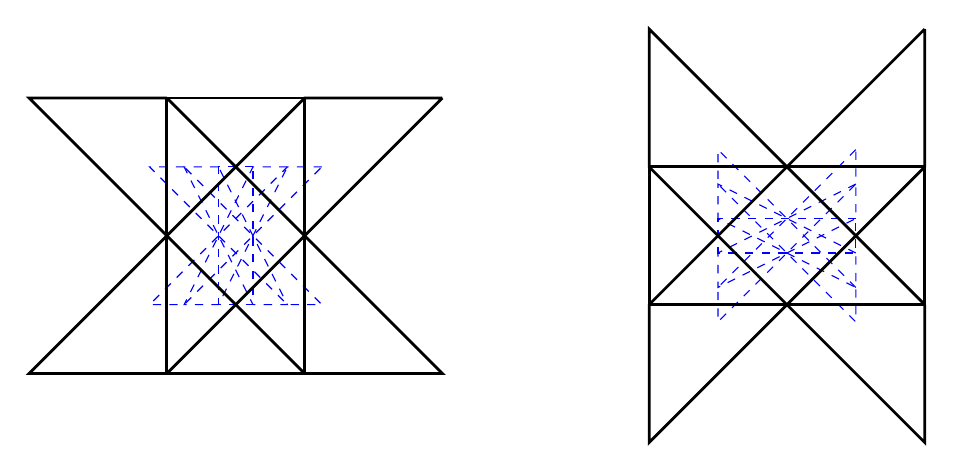
\begin{tikzpicture}[scale=3.5]
    \begin{scope}[scale=0.0625,shift={(-16,0)}]
    \begin{scope}[cm={1,0,-4,4,(0,0)}]
    \draw[dashed,color=blue] (1,1) -- (-1,1) -- (-1,-1) -- (1,-1) -- (1,1);
    \end{scope}
    \begin{scope}[cm={1,0,-2,4,(0,0)}]
    \draw[dashed,color=blue] (1,1) -- (-1,1) -- (-1,-1) -- (1,-1) -- (1,1);
    \end{scope}
    \begin{scope}[cm={1,0,0,4,(0,0)}]
    \draw[dashed,color=blue] (1,1) -- (-1,1) -- (-1,-1) -- (1,-1) -- (1,1);
    \end{scope}
    \begin{scope}[cm={1,0,2,4,(0,0)}]
    \draw[dashed,color=blue] (1,1) -- (-1,1) -- (-1,-1) -- (1,-1) -- (1,1);
    \end{scope}
    \begin{scope}[cm={1,0,4,4,(0,0)}]
    \draw[dashed,color=blue] (1,1) -- (-1,1) -- (-1,-1) -- (1,-1) -- (1,1);
    \end{scope}

    \begin{scope}[cm={4,0,-8,8,(0,0)}]
    \draw[line width=1pt] (1,1) -- (-1,1) -- (-1,-1) -- (1,-1) -- (1,1);
    \end{scope}
    \begin{scope}[cm={4,0,0,8,(0,0)}]
    \draw[line width=1pt] (1,1) -- (-1,1) -- (-1,-1) -- (1,-1) -- (1,1);
    \end{scope}
    \begin{scope}[cm={4,0,8,8,(0,0)}]
    \draw[line width=1pt] (1,1) -- (-1,1) -- (-1,-1) -- (1,-1) -- (1,1);
    \end{scope}
    \end{scope}

    \begin{scope}[scale=0.0625,shift={(16,0)}]
    \begin{scope}[cm={4,-4,0,1,(0,0)}]
    \draw[dashed,color=blue] (1,1) -- (-1,1) -- (-1,-1) -- (1,-1) -- (1,1);
    \end{scope}
    \begin{scope}[cm={4,-2,0,1,(0,0)}]
    \draw[dashed,color=blue] (1,1) -- (-1,1) -- (-1,-1) -- (1,-1) -- (1,1);
    \end{scope}
    \begin{scope}[cm={4,0,0,1,(0,0)}]
    \draw[dashed,color=blue] (1,1) -- (-1,1) -- (-1,-1) -- (1,-1) -- (1,1);
    \end{scope}
    \begin{scope}[cm={4,2,0,1,(0,0)}]
    \draw[dashed,color=blue] (1,1) -- (-1,1) -- (-1,-1) -- (1,-1) -- (1,1);
    \end{scope}
    \begin{scope}[cm={4,4,0,1,(0,0)}]
    \draw[dashed,color=blue] (1,1) -- (-1,1) -- (-1,-1) -- (1,-1) -- (1,1);
    \end{scope}

    \begin{scope}[cm={8,-8,0,4,(0,0)}]
    \draw[line width=1pt] (1,1) -- (-1,1) -- (-1,-1) -- (1,-1) -- (1,1);
    \end{scope}
    \begin{scope}[cm={8,0,0,4,(0,0)}]
    \draw[line width=1pt] (1,1) -- (-1,1) -- (-1,-1) -- (1,-1) -- (1,1);
    \end{scope}
    \begin{scope}[cm={8,8,0,4,(0,0)}]
    \draw[line width=1pt] (1,1) -- (-1,1) -- (-1,-1) -- (1,-1) -- (1,1);
    \end{scope}
    \end{scope}
\end{tikzpicture}
\caption{Shearlet supports for $s_x=4$ and $s_y=2$, showing levels $j=1$ (black) and $j=2$ (blue), on the left
for the up-down cone $r=0$ and on the right for the left-right cone $r=1$.}
\label{fig:shearlets}
\end{figure}

\begin{figure}
\centering
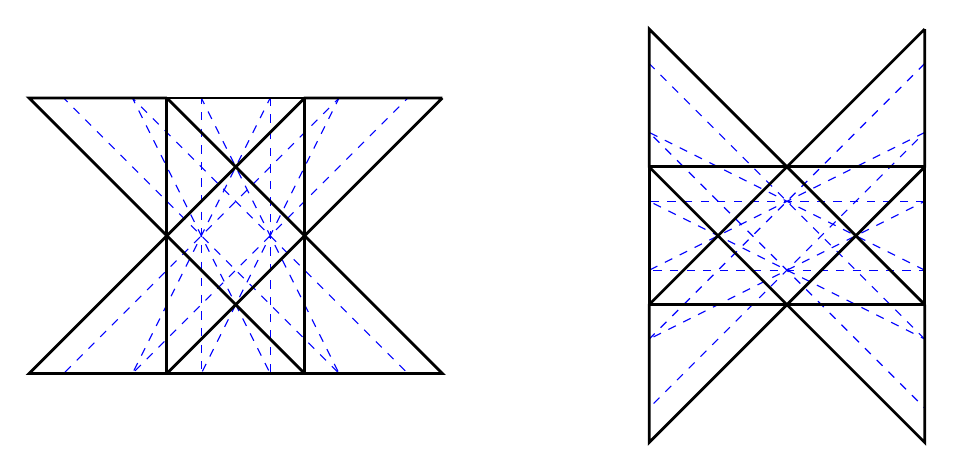
\begin{tikzpicture}[scale=1.75]
    \begin{scope}[scale=0.0625,shift={(-32,0)}]
    \begin{scope}[cm={4,0,-16,16,(0,0)}]
    \draw[dashed,color=blue] (1,1) -- (-1,1) -- (-1,-1) -- (1,-1) -- (1,1);
    \end{scope}
    \begin{scope}[cm={4,0,-8,16,(0,0)}]
    \draw[dashed,color=blue] (1,1) -- (-1,1) -- (-1,-1) -- (1,-1) -- (1,1);
    \end{scope}
    \begin{scope}[cm={4,0,0,16,(0,0)}]
    \draw[dashed,color=blue] (1,1) -- (-1,1) -- (-1,-1) -- (1,-1) -- (1,1);
    \end{scope}
    \begin{scope}[cm={4,0,8,16,(0,0)}]
    \draw[dashed,color=blue] (1,1) -- (-1,1) -- (-1,-1) -- (1,-1) -- (1,1);
    \end{scope}
    \begin{scope}[cm={4,0,16,16,(0,0)}]
    \draw[dashed,color=blue] (1,1) -- (-1,1) -- (-1,-1) -- (1,-1) -- (1,1);
    \end{scope}

    \begin{scope}[cm={8,0,-16,16,(0,0)}]
    \draw[line width=1pt] (1,1) -- (-1,1) -- (-1,-1) -- (1,-1) -- (1,1);
    \end{scope}
    \begin{scope}[cm={8,0,0,16,(0,0)}]
    \draw[line width=1pt] (1,1) -- (-1,1) -- (-1,-1) -- (1,-1) -- (1,1);
    \end{scope}
    \begin{scope}[cm={8,0,16,16,(0,0)}]
    \draw[line width=1pt] (1,1) -- (-1,1) -- (-1,-1) -- (1,-1) -- (1,1);
    \end{scope}
    \end{scope}

    \begin{scope}[scale=0.0625,shift={(32,0)}]
    \begin{scope}[cm={16,-16,0,4,(0,0)}]
    \draw[dashed,color=blue] (1,1) -- (-1,1) -- (-1,-1) -- (1,-1) -- (1,1);
    \end{scope}
    \begin{scope}[cm={16,-8,0,4,(0,0)}]
    \draw[dashed,color=blue] (1,1) -- (-1,1) -- (-1,-1) -- (1,-1) -- (1,1);
    \end{scope}
    \begin{scope}[cm={16,0,0,4,(0,0)}]
    \draw[dashed,color=blue] (1,1) -- (-1,1) -- (-1,-1) -- (1,-1) -- (1,1);
    \end{scope}
    \begin{scope}[cm={16,8,0,4,(0,0)}]
    \draw[dashed,color=blue] (1,1) -- (-1,1) -- (-1,-1) -- (1,-1) -- (1,1);
    \end{scope}
    \begin{scope}[cm={16,16,0,4,(0,0)}]
    \draw[dashed,color=blue] (1,1) -- (-1,1) -- (-1,-1) -- (1,-1) -- (1,1);
    \end{scope}

    \begin{scope}[cm={16,-16,0,8,(0,0)}]
    \draw[line width=1pt] (1,1) -- (-1,1) -- (-1,-1) -- (1,-1) -- (1,1);
    \end{scope}
    \begin{scope}[cm={16,0,0,8,(0,0)}]
    \draw[line width=1pt] (1,1) -- (-1,1) -- (-1,-1) -- (1,-1) -- (1,1);
    \end{scope}
    \begin{scope}[cm={16,16,0,8,(0,0)}]
    \draw[line width=1pt] (1,1) -- (-1,1) -- (-1,-1) -- (1,-1) -- (1,1);
    \end{scope}
    \end{scope}
\end{tikzpicture}
\caption{The same illustration as for Figure~\ref{fig:shearlets}, except with $s_x=2$, $s_y=1$.}
\label{fig:shearlets2}
\end{figure}

\subsection{The mother shearlets}

It remains only to consider the form of the mother shearlets. For our purposes it will suffice to consider
tensor products
\[
    \hPsi_m(\Bx) = \psi_m(x_1) \varphi_m(x_2).
\]
For levels $j>0$, $\psi_m$ will be wavelets, and $\varphi_m$ will be scaling functions\footnote{Functions with
low frequency content.}. Recall that $s_x>s_y$, so the behavior of $\psi$ will impact the behavior of the
transformed shearlet perpendicular to its principal direction (i.e. in the ``narrow'' direction), where it
will be wavelet-like, and correspondingly for $\varphi$ in the other direction.

In the following, the scaling functions and wavelets will be supported on
$[-\nicefrac{1}{2},\nicefrac{1}{2}]$, so that the produced shearlets for all levels $j \geq 0$ fit in the
domain $\Omega=[0,1]^2$ (assuming that the translations $\Bc$ are appropriately bounded).

The only scaling function we consider is the centered hat function
\[
    \varphi(z) = \begin{cases} 1-2|z|,& |z| < \frac{1}{2}, \\ 0,& \text{otherwise}. \end{cases}
\]
and our two principal wavelets can be defined in terms of it, as
\begin{align*}
    \psi_1(z) &= \varphi(2z) - \frac{1}{2} \varphi\left(2z-\frac{1}{2}\right)
                   - \frac{1}{2} \varphi\left(2z+\frac{1}{2}\right) \\
                   \psi_2(z) &= \frac{1}{2\sqrt{2}}
                   \left[\varphi\left(2z-\frac{1}{2}\right) - \varphi\left(2z+\frac{1}{2}\right)\right].
\end{align*}
See Figure~\ref{fig:wavelets}.

\begin{figure}
\centering
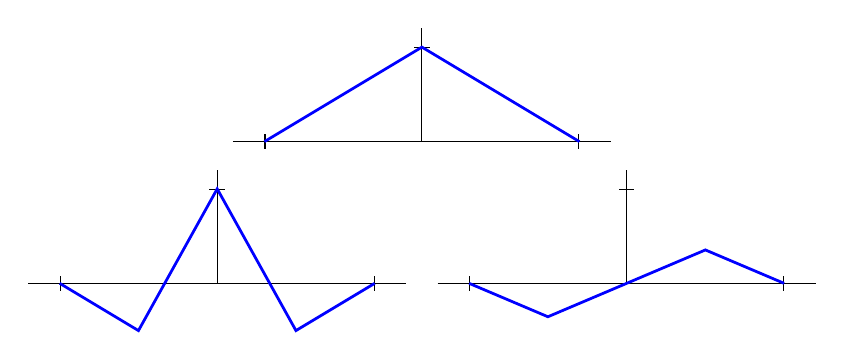
\begin{tikzpicture}[scale=4]
    \begin{scope}[yscale=0.3]
    \draw[|-|] (-0.5,0) -- (0.5,0); \draw[-|] (0,0) -- (0,1);
    \draw (-0.6,0) -- (-0.5,0); \draw (0.5,0) -- (0.6,0); \draw (0,1.0) -- (0,1.2);
    \draw[color=blue,line width=1pt] (-0.5,0) -- (0,1) -- (0.5,0);
    \end{scope}
    \begin{scope}[yscale=0.3,shift={(-0.65,-1.5)}]
    \draw[|-|] (-0.5,0) -- (0.5,0); \draw[-|] (0,0) -- (0,1);
    \draw (-0.6,0) -- (-0.5,0); \draw (0.5,0) -- (0.6,0); \draw (0,1.0) -- (0,1.2);
    \draw[color=blue,line width=1pt] (-0.5,0) -- (-0.25,-0.5) -- (0,1) -- (0.25,-0.5) -- (0.5,0);
    \end{scope}
    \begin{scope}[yscale=0.3,shift={(0.65,-1.5)}]
    \draw[|-|] (-0.5,0) -- (0.5,0); \draw[-|] (0,0) -- (0,1);
    \draw (-0.6,0) -- (-0.5,0); \draw (0.5,0) -- (0.6,0); \draw (0,1.0) -- (0,1.2);
    \draw[color=blue,line width=1pt] (-0.5,0) -- (-0.25,-0.3536) -- (0.25,0.3536) -- (0.5,0);
    \end{scope}
\end{tikzpicture}
\caption{Our scaling function (top) and two wavelets (bottom).}
\label{fig:wavelets}
\end{figure}

For the initial level $j=0$ we use scaling functions in {\em both} directions, so as to capture the
low-frequency components of the solution, i.e.
\[
    j=0 \implies \hPsi_0(\Bx) = \varphi(x_1) \varphi(x_2).
\]
This yields one mother shearlet for the first level and two for the remaining levels, all of which are
piece-wise bilinear, see Figure~\ref{fig:mothers}.

\begin{figure}
\centering
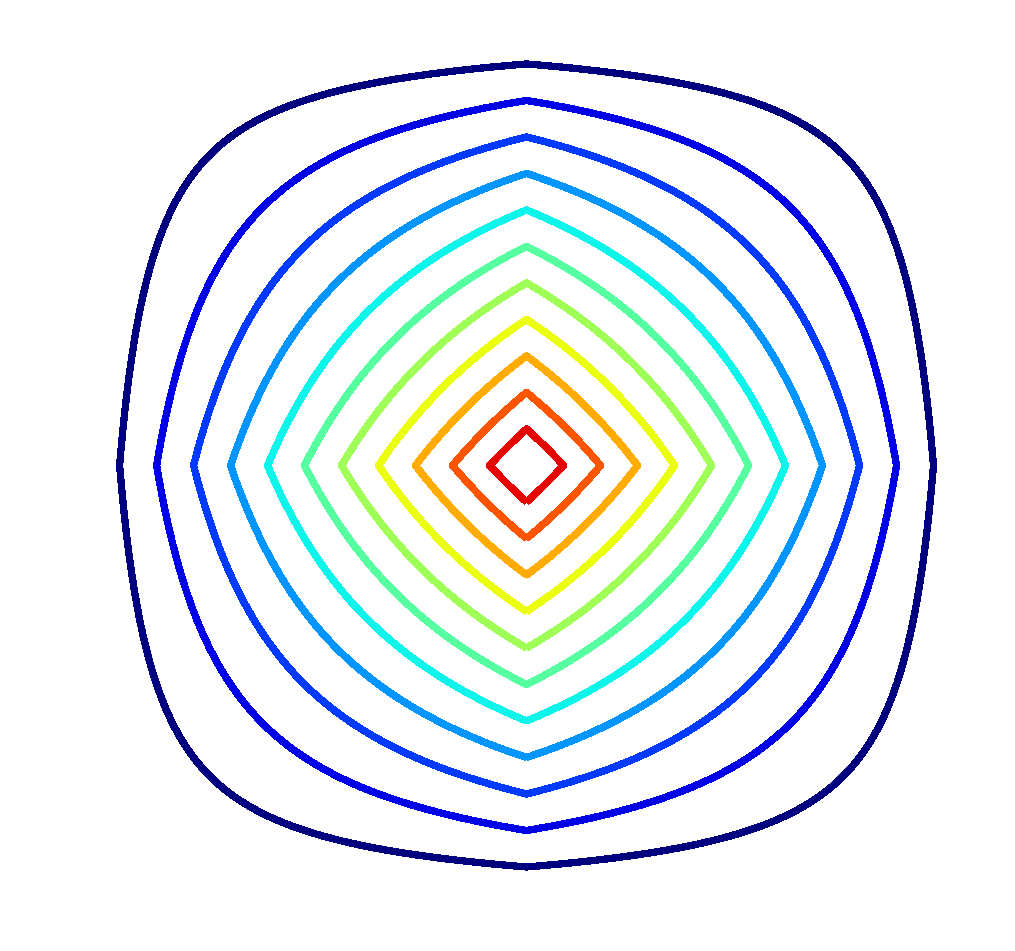
\includegraphics[width=5cm,height=5cm]{figs/shearlets/newmother0} \\
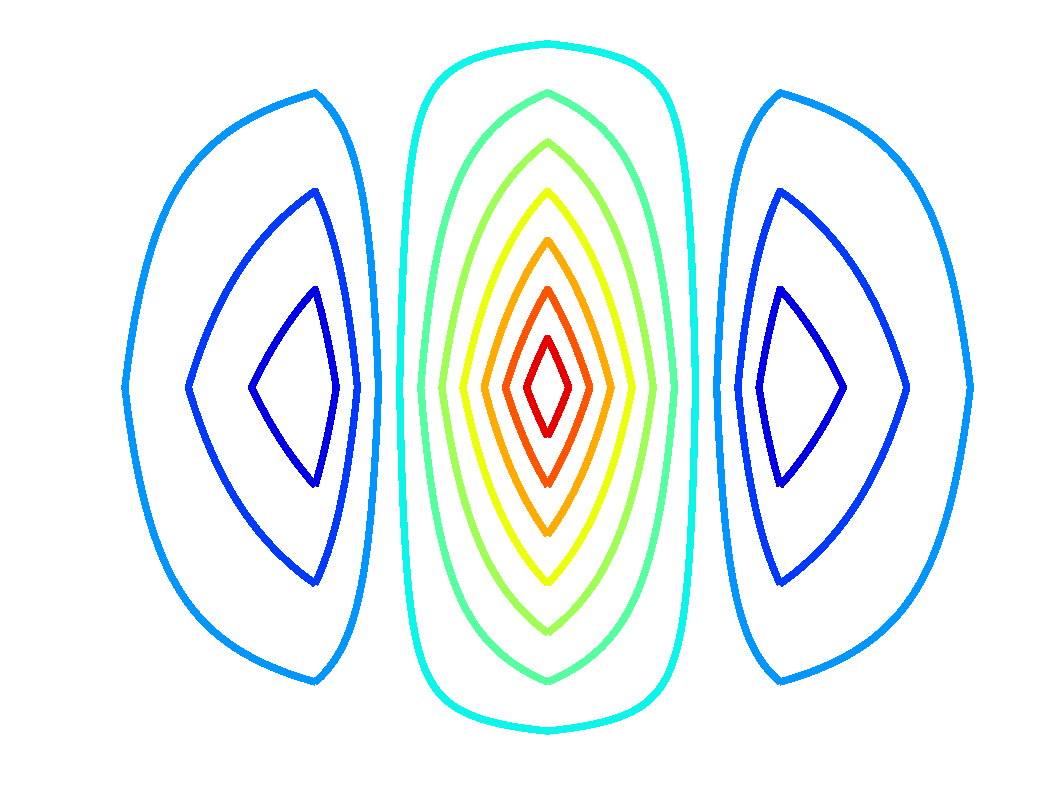
\includegraphics[width=5cm,height=5cm]{figs/shearlets/newmother1}
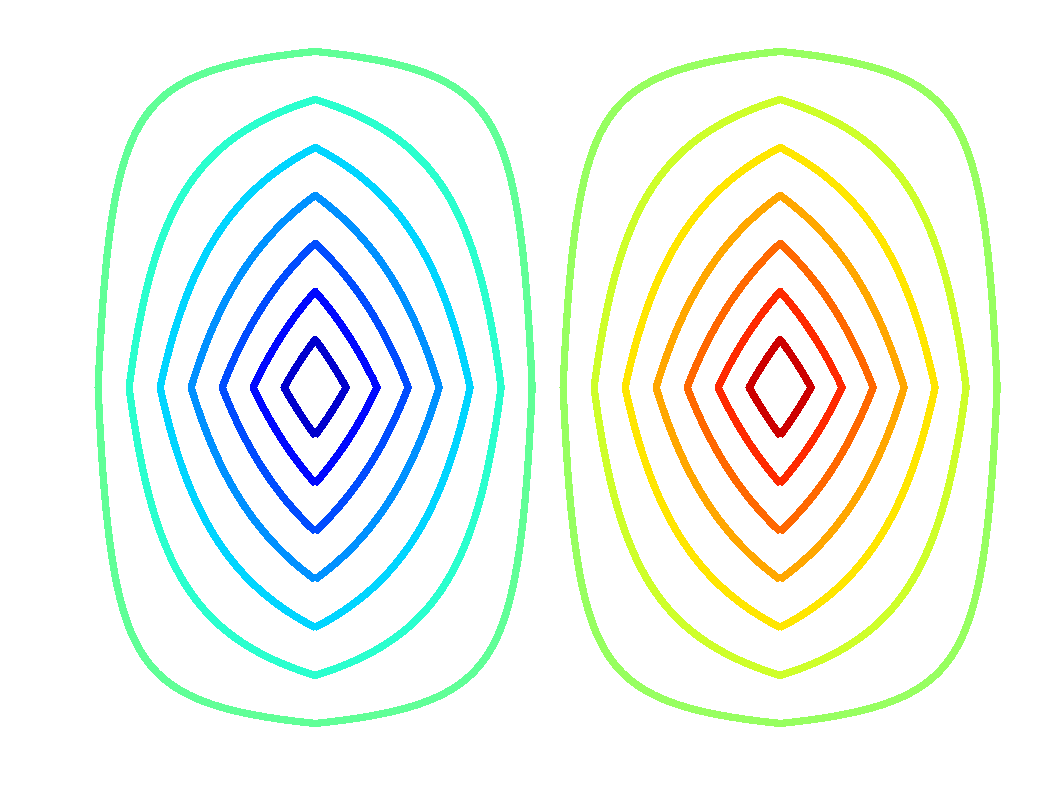
\includegraphics[width=5cm,height=5cm]{figs/shearlets/newmother2}
\caption{Mother shearlets for level $j=0$ (top) and $j>0$ (bottom).}
\label{fig:mothers}
\end{figure}

\subsection{Boundary conditions} \label{sec:boundarycond}

Since shearlets in general are not zero on the inflow boundary $\Gamma_-$, they cannot be used as-is to solve
\eqref{eqn:trp}. To remedy this, we introduce a multiplier function $z(\Bx)$ that is zero on $\Gamma_-$, and
nonzero everywhere else.

For the easiest test cases, namely constant transport directions $\Bv(\Bx)$, the construction of $z$ is
straightforward. We have, for example,
\[
    \Bv(\Bx) \equiv (1,1) 
    \implies \Gamma_- = [0,1] \times \{0\} \cup \{0\} \times [0,1]
    \quad \text{so} \quad
    z(\Bx) = x_1 x_2,
\]
or if $\Bv$ is aligned with one of the axes,
\[
    \Bv(\Bx) \equiv (0,1)
    \implies \Gamma_- = \{0\} \times [0,1]
    \quad \text{so} \quad
    z(\Bx) = x_2.
\]
It will not be necessary for us, and it is beyond the scope of this text, to pursue the construction of $z$
for more sophisticated cases. We mention, however, that it is desirable to keep $z$ as simple and smooth as
possible, both to preserve the approximating properties of shearlets and not to impose unreasonable conditions
on quadrature rules.

Once a suitable boundary multiplier function has been found, we simply substitute $z\Psi$ for every shearlet
$\Psi$, forming a new basis (for a different function space, a subspace of $V_0$) that conforms to the
boundary conditions. This treatment closely conforms to the partition of unity method (see \cite{Melenk96} and
\cite{Babuska97}).

We will also consider periodic boundary conditions, where this construction is unnecessary.

\subsection{Translations} \label{sec:translations}

It remains to specify the translation parameter $\Bc$. Assume that the fundamental wavelets and scaling
functions $\psi$ and $\varphi$ are piece-wise linear on a mesh with exactly $W_x$ and $W_y$ equally sized
intervals, respectively. That is,
\[
    \psi|_{\left(-\frac{1}{2}+\frac{i}{W_x},-\frac{1}{2}+\frac{i+1}{W_x}\right)}
    \qquad \text{and} \qquad
    \varphi|_{\left(-\frac{1}{2}+\frac{l}{W_y},-\frac{1}{2}+\frac{l+1}{W_y}\right)}
\]
are linear for all $0 \leq i < W_x$ and $0 \leq l < W_y$.

Now fix the level $j$ and let for the moment $k=0$. Then our shearlets $\aPsi{\cdot}{\cdot}{\cdot}{j}{0}$ are
piece-wise bilinear on a tensor product mesh which is uniform of resolution $\nicefrac{s_x^{-j}}{W_x}$ and
$\nicefrac{s_y^{-j}}{W_y}$ in the $x$- and $y$-directions respectively. If $s_x$ and $s_y$ are integers, this
mesh lines up perfectly with the boundaries of the domain.\footnote{If $s_x=\nicefrac{p}{q}$ is rational, the
mesh will also line up in the $x$-direction for those levels $j$ where $q^j$ divides $W_x$, if any (and
correspondingly in the $y$-direction.)}

As a consequence, we can represent all functions that are bilinear on this mesh by choosing translations
spaced by $\nicefrac{s_x^{-j}}{W_x}$ in the first direction, and $\nicefrac{s_y^{-j}}{W_y}$ in the second,
whence
\[
    \Bc \in \left\{\begin{pmatrix}
                    L(j) + \nicefrac{\alpha}{s_x^jW_x} \\ 
                    D(j) + \nicefrac{\beta}{s_y^jW_y}
                 \end{pmatrix} \;:\;
          0 \leq \alpha < R(j), \;\; 0 \leq \beta < U(j) \right\}.
\]
This set of translations is valid for the first cone $r=0$, and must be mirrored accordingly if $r=1$. It is
described by means of four helper functions: $(L(j), D(j))$ for the position of the ``bottom left'' shearlet,
and the maximal displacements $R(j)$ and $U(j)$ in each direction. These values are derived so that given any
level $j$, cone $r$ and translate $\Bc$, there is at least one shear $k$ so that $\aPsi{\cdot}{\Bc}{r}{j}{k}$
has support intersecting the domain $\Omega$. From this we find
\[ 
    L(j)=\begin{cases} \frac{s_x^{-j}}{W_x}-\frac{s_x^{-j} + s_y^{-j}}{2}, & j>0, \\ 0, & j=0, \end{cases}
    \qquad 
    R(j)=[1-2L(j)]s_x^jW_x+1,
\]
and
\[ 
    D(j) = 0,\qquad 
    U(j) = s_y^jW_y+1.
\]
We offer some illustrations in Figures~\ref{fig:extremeshearlets} and \ref{fig:translations} for the case
$W_x=4$, $W_y=4$ and $s_x=4$, $s_y=2$. 

For periodic boundary conditions, things become much simpler.
\[
    L(j) = D(j) = 0, \qquad R(j) = s_x^jW_x, \qquad U(j) = s_y^jW_y.
\]
Some care will be needed if the wavelets and scaling functions $\psi_\cdot$ and $\varphi_\cdot$ have different
structures (i.e. if $W_x$ and $W_y$ depend on $m$). Our construction does not allow coupling between the
translations $\Bc$ and the mother shearlets $m$. In this case, it would be most appropriate to let
$W_x=\lcm_m\{W_x(m)\}$ and $W_y=\lcm_m\{W_y(m)\}$ (least common multiple), so long as these numbers are not
prohibitively large.

\begin{figure}
\centering
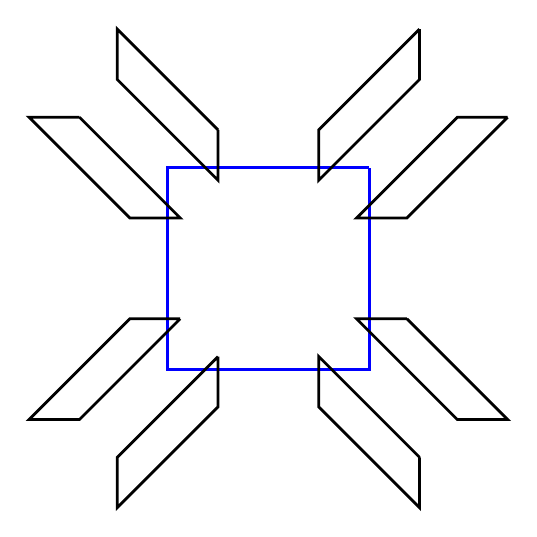
\begin{tikzpicture}[scale=4]
    \begin{scope}[scale=0.04]
    \begin{scope}[cm={8,0,0,8,(0,0)}]
    \draw[color=blue,line width=1pt] (1,1) -- (-1,1) -- (-1,-1) -- (1,-1) -- (1,1);
    \end{scope}
    \begin{scope}[cm={2,0,-4,4,(-13,8)}]
    \draw[line width=1pt] (1,1) -- (-1,1) -- (-1,-1) -- (1,-1) -- (1,1);
    \end{scope}
    \begin{scope}[cm={2,0,4,4,(13,8)}]
    \draw[line width=1pt] (1,1) -- (-1,1) -- (-1,-1) -- (1,-1) -- (1,1);
    \end{scope}
    \begin{scope}[cm={2,0,4,4,(-13,-8)}]
    \draw[line width=1pt] (1,1) -- (-1,1) -- (-1,-1) -- (1,-1) -- (1,1);
    \end{scope}
    \begin{scope}[cm={2,0,-4,4,(13,-8)}]
    \draw[line width=1pt] (1,1) -- (-1,1) -- (-1,-1) -- (1,-1) -- (1,1);
    \end{scope}
    \begin{scope}[cm={4,-4,0,2,(8,-13)}]
    \draw[line width=1pt] (1,1) -- (-1,1) -- (-1,-1) -- (1,-1) -- (1,1);
    \end{scope}
    \begin{scope}[cm={4,4,0,2,(8,13)}]
    \draw[line width=1pt] (1,1) -- (-1,1) -- (-1,-1) -- (1,-1) -- (1,1);
    \end{scope}
    \begin{scope}[cm={4,4,0,2,(-8,-13)}]
    \draw[line width=1pt] (1,1) -- (-1,1) -- (-1,-1) -- (1,-1) -- (1,1);
    \end{scope}
    \begin{scope}[cm={4,-4,0,2,(-8,13)}]
    \draw[line width=1pt] (1,1) -- (-1,1) -- (-1,-1) -- (1,-1) -- (1,1);
    \end{scope}
    \end{scope}
\end{tikzpicture}
\caption{The extreme shearlets for $j=1$, $s_x=4$, $s_y=2$. The blue square represents $\Omega$.}
\label{fig:extremeshearlets}
\end{figure}

\definecolor{purple}{rgb}{0.75,0,0.5}

\begin{figure}
\centering
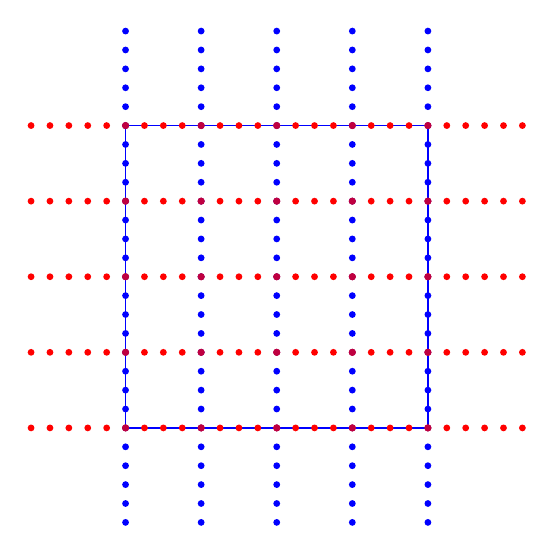
\begin{tikzpicture}[scale=4]
    \begin{scope}[scale=0.06]
    \begin{scope}[cm={8,0,0,8,(0,0)}]
    \draw[color=blue,line width=0.5pt] (1,1) -- (-1,1) -- (-1,-1) -- (1,-1) -- (1,1);
        \begin{scope}[scale=0.125]
            \foreach \x in {-13,-12,...,13} { \foreach \y in {-8,-4,...,8} { 
                \fill[color=red] (\x,\y) circle (0.18); 
                \fill[color=blue] (\y,\x) circle (0.18); 
            } }
            \foreach \x in {-8,-4,...,8} { \foreach \y in {-8,-4,...,8} {
                \fill[color=purple] (\x,\y) circle (0.19);
            } }
        \end{scope}
    \end{scope}
    \end{scope}
\end{tikzpicture} \\
\caption{Translation points for $j=1$, $s_x=4$, $s_y=2$, $W_x=4$, $W_y=2$. The red points are for $r=0$ and
the blue points are for $r=1$.}
\label{fig:translations} 
\end{figure}

\subsection{Numbers of shearlets}

Let us now consider the asymptotic complexity of this method by counting the number of shearlets $N(j)$ at
each level $j$. From the previous analysis, we get for $j>0$ (assuming $\nicefrac{s_x}{s_y}$ an integer):
\begin{multline*}
    N(j) = 2 M(j)
           \underbrace{\left(1+2\left(\frac{s_x}{s_y}\right)^{j-1}\right)}_{\text{shears}}
           \underbrace{\left(s_y^jW_y(j) + 1\right)}_{\text{up-down}} \\
           \underbrace{\left(\left(1+s_x^j\left(1+s_y^{-j}\right)\right)W_x(j)-1\right)}_{\text{left-right}}.
\end{multline*}
where $M(j)$ is the number of mother shearlets at level $j$, and $W_x(j)$ and $W_y(j)$ have the meaning given
in Section~\ref{sec:translations}. Thus, if $M,S,W$ are all asymptotically bounded, we obtain
\[
    N(j) \sim s_x^{2j},
\]
which, for the choices of $(s_x,s_y)$ listed earlier, reduces to rates of $16^j$ and $4^j$. The exact numbers
for levels $j=1,\ldots,6$ are listed in Table~\ref{tbl:numlets}, given the previously described mother
shearlets---that is, $M(0)=1$ and $M(j)=2$ for $j>0$.

Of course, this is an extremely rapid growth. Performing a full space solution with even very modest
resolution $j$ is quite challenging, not only due to solving the linear system, but also because assembly is a
nontrivial problem (as we shall see). The main hope for shearlets lie in their naturally adaptive properties.
One might hope that most active coefficients belong to shearlets which are aligned with the transport
direction $\Bv(\Bx)$, so that the vast majority of the search space can be dispensed with.

\begin{table}
\centering
\def\arraystretch{1.4}
\begin{tabular}{r@{\qquad}l@{\qquad}l}
$j$ & $(4,2)$ & $(2,1)$ \\
\hline $1$ & $8.10\cdot10^{2}M(1)$ & $3.42\cdot10^{2}M(1)$ \\
\hline $2$ & $7.47\cdot10^{3}M(2)$ & $1.05\cdot10^{3}M(2)$ \\
\hline $3$ & $8.90\cdot10^{4}M(3)$ & $3.62\cdot10^{3}M(3)$ \\
\hline $4$ & $1.22\cdot10^{6}M(4)$ & $1.34\cdot10^{4}M(4)$ \\
\hline $5$ & $1.81\cdot10^{7}M(5)$ & $5.13\cdot10^{4}M(5)$ \\
\hline $6$ & $2.79\cdot10^{8}M(6)$ & $2.01\cdot10^{5}M(6)$ \\
\end{tabular}
\caption{Number of shearlets per level. $(s_x,s_y)=(4,2)$ on the left and $(s_x,s_y)=(2,1)$ on the right. In
both cases, $W_x(j)=2$ and $W_y(j)=4$.} \label{tbl:numlets}
\end{table}

\section{Algorithms} \label{sec:algorithms}

In the following, we will describe in some detail a basic implementation for a shearlet solver for
\eqref{eqn:trp}. There are no significant new ideas here, but it will perhaps serve to highlight some typical
difficulties faced.

At the time this work was done, this was the only shearlet implementation available intended for the solution
of PDEs. Since then, other work has shown promise using different strategies, among them \cite{ObermeierXX}.

\subsection{Numbering}

We number shearlets according to a hierarchy of parameters. As the only open-ended parameter, and since the
ranges of other parameters depend on it, naturally $j$ must be most significant. The order of the others is
not overly important.

In the following, we will describe shearlets in algorithms as a single variable (usually $s$ or $t$), which
can be assumed to work as a structure, and that sub-fields can be accessed by dot-notation such as $s.j$. We
will also speak of $s$ as the shearlet itself (i.e. the mathematical function). The meaning should in either
case be clear from the context.

\subsection{Transformation} \label{sec:transformation}

For our purposes we need to be able to evaluate shearlets at arbitrary points in $\bbR^2$. This is done using
the transformation technique in \eqref{eqn:trflet}. A function called $\basetrf$ takes a shearlet and produces
the transformation matrix $\BA$ and the translation vector $\Bc$,
\[ 
    (\BA,\Bc) \leftarrow \basetrf(s).
\]
The mapping $\Bx \mapsto \BA(\Bx-\Bc)$ is an affine transformation mapping the square
$[-\nicefrac{1}{2},\nicefrac{1}{2}]^2$ to the support of $s$.

The reason for the name $\basetrf$ is that it will also be useful to have a more general function called
$\trf$ that can produce mappings into subdomains of the support of $s$. Recall that $s$ is defined as an
affine transformation of a tensor product of two piece-wise linear functions, so that $s$ is piece-wise
polynomial with maximal degree $2$. (It is not necessarily piece-wise bilinear, because the shearing will add
squared terms.) By {\em subdomain} we mean the subsets of the support of $s$ on which $s$ is polynomial. These
are numbered as shown in Figure~\ref{fig:subnumbering}.

\begin{figure}
\centering
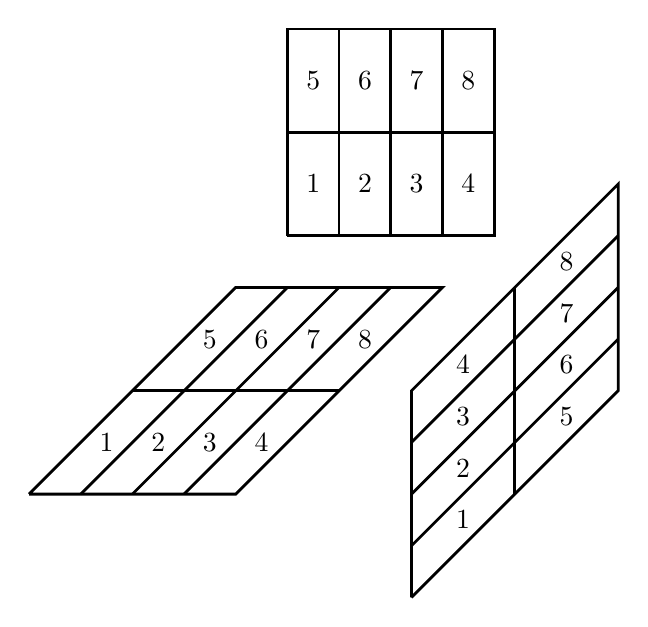
\begin{tikzpicture}[scale=1.3125]
    \draw[line width=1pt] (-1,-1) -- (1,-1) -- (1,1) -- (-1,1) -- (-1,-1);
    \draw[line width=1pt] (-0.5,-1) -- (-0.5,1);
    \draw[line width=1pt] (0,-1) -- (0,1);
    \draw[line width=1pt] (0.5,-1) -- (0.5,1);
    \draw[line width=1pt] (-1,0) -- (1,0);
    \node at (-0.75,-0.5) {1}; \node at (-0.25,-0.5) {2}; \node at (0.25,-0.5) {3}; \node at (0.75,-0.5) {4};
    \node at (-0.75,0.5) {5}; \node at (-0.25,0.5) {6}; \node at (0.25,0.5) {7}; \node at (0.75,0.5) {8};
    \begin{scope}[cm={1,0,1,1,(-1.5,-2.5)}]
        \draw[line width=1pt] (-1,-1) -- (1,-1) -- (1,1) -- (-1,1) -- (-1,-1);
        \draw[line width=1pt] (-0.5,-1) -- (-0.5,1);
        \draw[line width=1pt] (0,-1) -- (0,1);
        \draw[line width=1pt] (0.5,-1) -- (0.5,1);
        \draw[line width=1pt] (-1,0) -- (1,0);
        \node at (-0.75,-0.5) {1}; \node at (-0.25,-0.5) {2}; \node at (0.25,-0.5) {3}; \node at (0.75,-0.5) {4};
        \node at (-0.75,0.5) {5}; \node at (-0.25,0.5) {6}; \node at (0.25,0.5) {7}; \node at (0.75,0.5) {8};
    \end{scope}
    \begin{scope}[cm={0,1,1,1,(1.2,-2.5)}]
        \draw[line width=1pt] (-1,-1) -- (1,-1) -- (1,1) -- (-1,1) -- (-1,-1);
        \draw[line width=1pt] (-0.5,-1) -- (-0.5,1);
        \draw[line width=1pt] (0,-1) -- (0,1);
        \draw[line width=1pt] (0.5,-1) -- (0.5,1);
        \draw[line width=1pt] (-1,0) -- (1,0);
        \node at (-0.75,-0.5) {1}; \node at (-0.25,-0.5) {2}; \node at (0.25,-0.5) {3}; \node at (0.75,-0.5) {4};
        \node at (-0.75,0.5) {5}; \node at (-0.25,0.5) {6}; \node at (0.25,0.5) {7}; \node at (0.75,0.5) {8};
    \end{scope}
\end{tikzpicture}
\caption{An example of subdomain numbering, where $W_x=4$ and $W_y=2$. The resulting shearlets are piece-wise
polynomial on $W_xW_y=8$ sections.} \label{fig:subnumbering}
\end{figure}

Thus we define a function $\trf(s,i)$ which takes a subdomain number as a second optional argument. If $i$ is
not specified or $i=0$, it is assumed that $\basetrf(s)$ is meant. See Algorithm \ref{alg:trf}.

\begin{algorithm}
\caption{$\trf$ computes $\BA$ and $\Bc$ for a given shearlet and subdomain number.} \label{alg:trf}
\begin{algorithmic}[1]
\REQUIRE Shearlet $s$ and optional subdomain number $0\leq i\leq 8$
\STATE $(\BA,\Bc)\leftarrow \basetrf(s)$
\IF{$i$ is given and $i>0$}
\STATE $\Bd\leftarrow \left(\frac{1}{W_x}\left(\left(i-1\modd W_x\right)+\frac{1}{2}\right)-\frac{1}{2},\quad
        \frac{1}{W_y}\left(\lfloor\frac{i-1}{W_x}\rfloor+\frac{1}{2}\right)-\frac{1}{2}\right)^\intercal$
\STATE $\Bc\leftarrow \BA^{-1}\Bd+\Bc$
\STATE $\BA\leftarrow \begin{pmatrix} W_x&\\&W_y \end{pmatrix} \cdot \BA$
\ENDIF
\RETURN $(\BA,\Bc)$
\end{algorithmic}
\end{algorithm}

In the following, we will often be concerned with the polygon defined by the support of a given shearlet, or
one of its subdomains. We will consider polygons as $2\times n$-matrices of vertices $(p_1,p_2,\ldots,p_n)$
numbered counterclockwise, where $p_n\neq p_1$. A useful convenience is the function $\corners$, which
computes these vertices by transforming the corners of the reference square $[-1/2,1/2]^2$, see Algorithm
\ref{alg:corners}. If no shearlet is given, it returns the corners of the computational domain.

\begin{algorithm}
\caption{$\corners$ computes the vertices of a shearlet support or subdomain.} \label{alg:corners}
\begin{algorithmic}[1]
\REQUIRE Optional shearlet $s$ and optional subdomain number $0\leq i\leq 8$
\IF {$s$ is not given}
\RETURN $\begin{pmatrix} 0&1&1&0 \\ 0&0&1&1 \end{pmatrix}$
\ENDIF
\STATE $(\BA,\Bc)\leftarrow \trf(s,i)$
\STATE $\Bp\leftarrow \frac{1}{2} \BA^{-1}\begin{pmatrix} -1&1&1&-1 \\ -1&-1&1&1 \end{pmatrix} + \Bc$
\IF {$s.r=1$}
\STATE Reverse the order of $\Bp$
\ENDIF
\RETURN $\Bp$
\end{algorithmic}
\end{algorithm}

\subsection{Assembly strategy} \label{ssec:assemblystrat}

\subsubsection{Stiffness matrix}

Given a bilinear form $\blfa(\cdot,\cdot)$ we want to compute the corresponding stiffness matrix for a given
index set $\cI$ of shearlets. In an ordinary hierarchical setting (e.g. with hat functions), one would rely on
a {\em refinement relation} that expresses a function as a linear combination of functions on the next level.
This would allow us to compute the stiffness matrix for the highest level only, and then use the refinement
relation to fill out the coarser matrices. There are several problems with this.

\begin{enumerate}
\item The number of shearlets on each level increases very fast, asymptotically (in our worst case) $16^j$,
compared to the more conventional $4^j$. The saved effort from not having to directly calculate the coarse
levels becomes almost negligible.

\item In a more traditional setting, such as with triangular elements and hat functions, it is possible to
assemble the matrix in time that scales linearly with the number of elements, as this circumvents the
necessity of having to check if the supports of two functions overlap. No such shortcut is readily available
to us in the shearlet case.\footnote{It is true that there are simple methods that can identify a number of
negatives (no intersection), such as checking the center and diameter of shearlet supports, or cheap
intersection checking routines. However, these cases still have to be {\em tested}, and moreover, the
stiffness matrix will nevertheless not be sparse (although it might be compressible).}

\item The primary motivation for implementing a shearlet basis/frame is to employ adaptive methods, and thus
to be able to dispense with a large number of fine-level basis functions. The refinement relation strategy
outlined would negate to some extent the advantages offered by adaptivity.
\end{enumerate}

Due to this, for the time being, we will fall back to the primitive loop which merely iterates over all pairs
of shearlets and computes their corresponding matrix entry. Some speedup is possible in this step since our
matrix is symmetric. Parallelization ought to be considered here.

How, then, do we go about computing $\blfa(s_i,s_j)$? The most obvious approach is straightforward.

\begin{enumerate}
\item Identify the vertices of the supports of $s_i$ and $s_j$ using the function $\corners$.
\item Check if the supports intersect. If they do not, return $0$.
\item If the supports intersect, loop over pairs of subdomains of the supports of $s_i$ and $s_j$. Compute
the intersection of this pair if it is nonempty. This produces a set of nonempty disjoint polygons $P_k$
whose union is the intersection of supports of $s_i$ and $s_j$, and which has the property that both $s_i$ and
$s_j$ are polynomial on any $P_k$.
\item Further divide each $P_k$ into a set of triangles. On each triangle, form a quadrature rule. Take the
union of these quadrature rules as a quadrature rule for the intersection of the supports of $s_i$ and $s_j$.
\end{enumerate}

Once the quadrature rule is in hand, the integrand of the bilinear form $\blfa$ can be evaluated on the
quadrature points and summed up accordingly.

There should be a basic choice of quadrature rule defined on a reference triangle, which can then be
transformed.  This part is essentially identical to triangular Lagrangian FEM. If there are no variable
coefficients, we can achieve exact integration with a quadrature rule of sufficiently high order. If there
{\em are} variable coefficients, the case becomes a little more complicated, which we discuss in
Section~\ref{sec:error-in-quadrature}.

This strategy relies heavily on reliable routines for checking and computing intersections between convex
polygons. Experiments suggest that most of the processing time is spent doing operations like these, and care
should be taken to implement these properly (see Section~\ref{sec:intersections}).\footnote{There is a fair
amount of overlap available. For example if $s_i$ and $s_j$ give rise to a quadrature rule $q$, then
translates of $s_i$ and $s_j$ (by the same vector) give rise to translates of $q$, unless these translates
intersect with the boundary of the domain.}

We now assume the existence of these functions:

\begin{enumerate}
\item A function $\checkintersection(s,t)$ for checking if the supports of shearlets $s$ and $t$ intersect at
all.
\item A function $\computeintersection(p,q)$ for computing intersections between two convex polygons $p$ and
$q$.
\item A function $\splitpolygon(p)$ for reducing a polygon $p$ to a collection of triangles.
\item A function $\transformquadrule(q,p)$ for transforming a quadrature rule $q$ defined on a reference
triangle onto the triangle $p$.
\end{enumerate}

The algorithms for checking and computing intersections are discussed further in
Section~\ref{sec:intersections}. The $\splitpolygon$ function can be implemented in a myriad of different
ways, one of which is described in Algorithm~\ref{alg:splitpolygon}. This algorithm splits a polygon as shown
in Figure~\ref{fig:splitpolygon}, where the red vertex is vertex number $1$. The algorithm alternates between
adding a triangle on the ``right'' or ``left'' side, and keeps track of the next unused vertex on both sides.
No new vertices are introduced.

Algorithm~\ref{alg:builddquadrule} contains pseudo-code for the $\builddquadrule$ function, which builds a
quadrature rule for the intersection of two shearlet supports. 

\begin{figure}
\centering
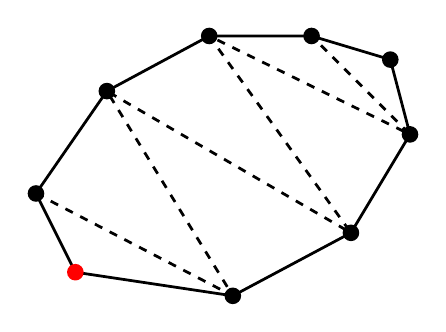
\begin{tikzpicture}
    \coordinate (p1) at (0,0);
    \coordinate (p2) at (2,-0.3);
    \coordinate (p3) at (3.5,0.5);
    \coordinate (p4) at (4.25,1.75);
    \coordinate (p5) at (4,2.7);
    \coordinate (p6) at (3,3);
    \coordinate (p7) at (1.7,3);
    \coordinate (p8) at (0.4,2.3);
    \coordinate (p9) at (-0.5,1);
    \draw[line width=1pt] (p1) -- (p2) -- (p3) -- (p4) -- (p5) -- (p6) -- (p7) -- (p8) -- (p9) -- (p1);
    \fill[color=red] (p1) circle (3pt);
    \fill (p2) circle (3pt); \fill (p3) circle (3pt); \fill (p4) circle (3pt); \fill (p5) circle (3pt); 
    \fill (p6) circle (3pt); \fill (p7) circle (3pt); \fill (p8) circle (3pt); \fill (p9) circle (3pt);
    \draw[dashed, line width=1pt] (p9) -- (p2) -- (p8) -- (p3) -- (p7) -- (p4) -- (p6);
\end{tikzpicture}
\caption{Splitting a polygon into triangles. The red vertex is number one.} \label{fig:splitpolygon}
\end{figure}

\begin{algorithm}
\caption{$\splitpolygon$ divides a polygon $p$ into a collection of triangles.}
\label{alg:splitpolygon}
\begin{algorithmic}[1]
\REQUIRE $2\times N$ matrix $p$ denoting a polygon
\STATE start\ $\leftarrow3$, end\ $\leftarrow1$, right\ $\leftarrow$\ false, $T\leftarrow \left\{\begin{pmatrix}
p_{\cdot,1}&p_{\cdot,2}&p_{\cdot,N} \end{pmatrix}\right\}$ \WHILE{$\mathrm{start}+\mathrm{end}\leq N$}
\IF{right}
\STATE $T\leftarrow T\cup\left\{\begin{pmatrix}
p_{\cdot,\mathrm{start}-1}&p_{\cdot,\mathrm{start}}&p_{\cdot,N-\mathrm{end}+1} \end{pmatrix}\right\}$
\STATE $\text{start} \leftarrow \text{start} + 1$
\ELSE
\STATE $T\leftarrow T\cup\left\{\begin{pmatrix}
p_{\cdot,\mathrm{start}-1}&p_{\cdot,N-\mathrm{end}}&p_{\cdot,N-\mathrm{end}+1} \end{pmatrix}\right\}$
\STATE $\text{end} \leftarrow \text{end} + 1$
\ENDIF
\STATE $\text{right} \leftarrow \neg\text{right}$
\ENDWHILE
\end{algorithmic}
\end{algorithm}

\begin{algorithm}
\caption{$\builddquadrule$ constructs a quadrature rule for the intersection of the supports of two shearlets
$s$ and $t$.}
\label{alg:builddquadrule}
\begin{algorithmic}[1]
\REQUIRE Shearlets $s$, $t$ and basic quadrature rule $q$
\STATE $r\leftarrow \emptyset$
\FOR {$i,j\in\{1,\ldots,8\}$}
\STATE $p\leftarrow\corners(s,i)$
\STATE $q\leftarrow\corners(t,j)$
\STATE $B\leftarrow\splitpolygon(\computeintersection(p,q))$
\FOR {$c\in B$}
\STATE $r\leftarrow r\cup\left\{\transformquadrule(q,c)\right\}$
\ENDFOR
\ENDFOR
\end{algorithmic}
\end{algorithm}

%\begin{algorithm}
%\caption{{$\evalblf$} evaluates a bilinear form.} \label{alg:evalblf}
%\begin{algorithmic}[1]
%\REQUIRE Shearlets $s$, $t$, basic quadrature rule $q$ and a function $f(s,t,x)$ for evaluating the integrand
%of a bilinear form at a point $x$.
%\IF {$\checkintersection(s,t)$}
%\STATE $q\leftarrow\builddquadrule(s,t,q)$
%\STATE $r\leftarrow 0$
%\FOR {quadrature point $x$ with weight $w$ $\in q$}
%\STATE $r\leftarrow r+w\cdot f(s,t,x)$
%\ENDFOR
%\RETURN r
%\ELSE
%\RETURN 0
%\ENDIF
%\end{algorithmic}
%\end{algorithm}

\subsubsection{Load vector}

For evaluating the right hand side load vector $\lfl(\cdot)$ the strategy is mostly the same, except we can
ignore most of the intersection checking. The function $\buildsquadrule$ mirrors $\builddquadrule$, and its
pseudo-code is presented in Algorithm~\ref{alg:buildsquadrule}.

\begin{algorithm}
\caption{$\buildsquadrule$ constructs a quadrature rule for the support of a shearlet $s$.}
\label{alg:buildsquadrule}
\begin{algorithmic}[1]
\REQUIRE Shearlet $s$ and basic quadrature rule $q$
\STATE $r\leftarrow \emptyset$
\FOR {$i\in\{1,\ldots,8\}$}
\STATE $p\leftarrow\corners(s,i)$
\STATE $B\leftarrow\splitpolygon(p)$
\FOR {$c\in B$}
\STATE $r\leftarrow r\cup\transformquadrule(q,c)$
\ENDFOR
\ENDFOR
\end{algorithmic}
\end{algorithm}

%\begin{algorithm}
%\caption{{$\evallf$} evaluates a linear form.} \label{alg:evallf}
%\begin{algorithmic}[1]
%\REQUIRE Shearlet $s$, basic quadrature rule $q$ and a function $f(s,x)$ for evaluating the integrand of a
%bilinear form at a point $x$.
%\STATE $q\leftarrow\buildsquadrule(s,q)$
%\STATE $r\leftarrow 0$
%\FOR {quadrature point $x$ with weight $w$ $\in q$}
%\STATE $r\leftarrow r+w\cdot f(s,x)$
%\ENDFOR
%\RETURN r
%\end{algorithmic}
%\end{algorithm}

\subsubsection{Intersections} \label{sec:intersections}

Our method relies on computing intersections between many different polygons, or deciding if polygons are
disjoint. There are several algorithms for computing and detecting intersections, see for example
\cite{Toussaint85, Rourke82, Chazelle80}.  These all assume convexity, which is valid in\
our case.

For checking disjointedness, we rely on the {\em separating axis theorem}, which is commonly used in game
programming for collision detection \cite{Gottschalk96}.

\begin{theorem}[Separating Axis Theorem (SAT)] \label{thm:sat}
Let $A,B\subseteq\bbR^2$ be convex sets in $\bbR^2$. Then $A \cap B=\emptyset$ if and only if there exists a
line that separates $A$ from $B$. Moreover, if $A$ and $B$ are polygons with empty intersection, such a
separating line can always be found among the extensions of the edges of $A$ and $B$.
\end{theorem}
\begin{proof}
The first statement is the Hahn-Banach theorem. For the other, assume that $A$ and $B$ are disjoint convex
polygons, and let $\Ba$, $\Bb$ be points of minimal distance between them. If either $\Ba$ or $\Bb$ is not a
vertex, they are points on edges, and the extensions of either of these edges yield a separating line. 

If both $\Ba$ and $\Bb$ are vertices, consider vertex $\Ba$ and the extension of its edges dividing the
space outside of $A$ into three regions as shown in Figure~\ref{fig:sat}, two of which are named $U$ and $L$.
Assume vertex $\Bb$ is not in $L$. 

If none of $B$ intersects $L$, the edge $r$ will be a separating line. If not, define the line $h$ through
$\Bb$ as being parallel to $r$, and the line $g$ through $\Bb$ as being orthogonal to the line through $\Ba$
and $\Bb$. Now, consider the edge from $\Bb$ in the direction of $L$. Since $B$ intersects $L$ and $\Bb$ is
the point of $B$ closest to $A$, this edge must lie in the wedge between lines $h$ and $g$, and so it clearly
gives a separating line. Moreover, if this wedge is empty, we can see that this contradicts the assumption
that $\Bb$ is closest to $A$.

If $\Bb$ is in $L$, it is not in $U$, and the argument works correspondingly.
\end{proof}

\begin{figure}
\centering
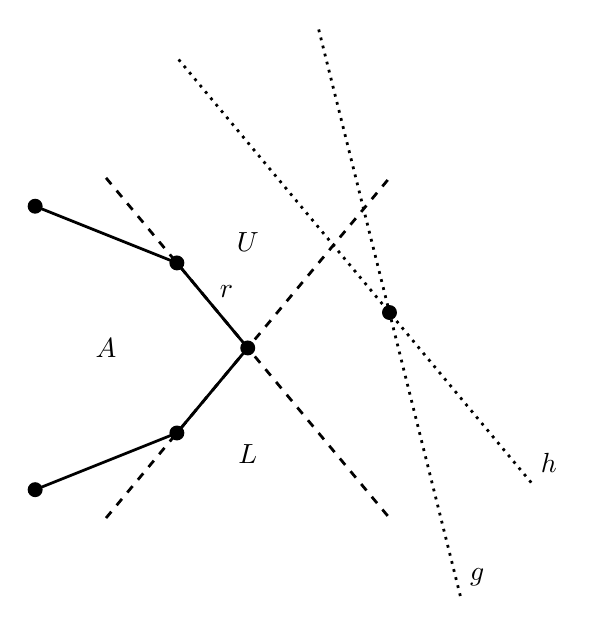
\begin{tikzpicture}[scale=0.9]
    \coordinate (a1) at (0,2); \coordinate (a4) at (0,-2);
    \coordinate (a2) at (2,1.2); \coordinate (a2far) at (5,-2.4); \coordinate (a2near) at (1,2.4);
    \coordinate (a3) at (2,-1.2); \coordinate (a3far) at (5,2.4); \coordinate (a3near) at (1,-2.4);
    \coordinate (hfar) at (2,4.1); \coordinate[label=45:$h$] (hnear) at (7,-1.9);
    \coordinate (gfar) at (4,4.5); \coordinate[label=45:$g$] (gnear) at (6,-3.5);
    \coordinate[label={[label distance=3pt]180:$\Ba$}] (a) at (3,0);
    \coordinate[label={[label distance=3pt]0:$\Bb$}] (b) at (5,0.5);
    \draw[line width=1pt] (a1) -- (a2) -- (a) -- (a3) -- (a4);
    \fill (a1) circle (3pt); \fill (a2) circle (3pt); \fill (a) circle (3pt);
    \fill (a3) circle (3pt); \fill (a4) circle (3pt); \fill (b) circle (3pt);
    \draw[dashed, line width=1pt] (a2near) -- (a2far);
    \draw[dashed, line width=1pt] (a3near) -- (a3far);
    \draw[dotted, line width=1pt] (hnear) -- (hfar);
    \draw[dotted, line width=1pt] (gnear) -- (gfar);
    \node at (1,0) {$A$}; \node at (3,-1.5) {$L$}; \node at (3,1.5) {$U$};
    \node at (2.7,0.8) {$r$};
\end{tikzpicture}
\caption{The separating axis theorem (Theorem~\ref{thm:sat}.)} \label{fig:sat}
\end{figure}

The consequence of Theorem~\ref{thm:sat} is that we can decide if two polygons $p$ and $q$ are disjoint by
looping through the edges of one of them (say $p$). If the vertices are ordered counterclockwise, and we
assume that an edge $e$ therefore has a counterclockwise ``direction'', we already know that $p$ lies on the
left side of $e$, so we need only check if $q$ lies entirely on the right, which can be done by checking the
vertices of $q$ (again, because of convexity). At this point, if no separating line has been found, one has to
loop through the edges of $q$ in a similar fashion.

This is expressed in Algorithm~\ref{alg:checkintersection}. Note that it does not actually check if the
polygons intersect in the computational domain. A few false positives do not worry us, however.

\begin{algorithm}
\caption{$\checkintersection$ checks if the supports of two shearlets $s$ and $t$ are disjoint or not. Returns
true if the supports intersect.}
\label{alg:checkintersection}
\begin{algorithmic}[1]
\REQUIRE Shearlets $s$ and $t$
\STATE $p\leftarrow\corners(s)$, $q\leftarrow\corners(t)$
\FOR{$e\in\mathrm{Edges}(p)$} \label{alg:ci:outer}
\STATE $\text{separatingLine}\leftarrow\mathrm{true}$
\FOR{$\Bv\in\mathrm{Vertices}(q)$}
\IF{$\Bv$ is on the left side of $e$}
\STATE $\text{separatingLine}\leftarrow\mathrm{false}$
\BREAK
\ENDIF
\ENDFOR
\IF{\text{separatingLine}}
\RETURN false
\ENDIF
\ENDFOR
\STATE Repeat loop from line \ref{alg:ci:outer} with $p$ and $q$ interchanged
\RETURN true
\end{algorithmic}
\end{algorithm}

For actually {\em computing} the intersection between two polygons we have employed the General Polygon
Clipper (GPC) library from the University of Manchester \cite{GPC}.

For the case of periodic boundary conditions, some more work is needed. Two shearlets that do not intersect in
the non-periodic case can nevertheless intersect if they are periodically extended. For checking the
intersection, it is necessary to translate the domain of the shearlets by $(m,n)$,
$m,n\in\left\{-1,0,1\right\}$, which corresponds to a shift of at most one period in either direction. This
range of $m,n$ can be restricted somewhat if we take into account the diameters of the shearlet supports, and
where the supports are located with respect to one another. For the smallest shearlets, it will be possible to
reduce the number of translations to be checked to one. Also note that in the periodic case there are no false
positives, as {\em every} possible point of intersection is ``in'' the domain.

For computing the intersection in the periodic case, we must construct unions of polygons, which is supported
by GPC.  Given the support of a shearlet, we intersect it, and all its relevant translations, with the
computational domain. This gives us a union of polygons in $[0,1]^2$ representing the support of that
shearlet. Two such unions can be intersected with GPC and the result is also a union of polygons.

\subsubsection{Error in quadrature} \label{sec:error-in-quadrature}

If the bilinear form $\blfa$ does not contain variable coefficients, it will normally be possible to evaluate
the stiffness matrix exactly (up to machine precision) by choosing a basic quadrature rule which is strong
enough. This will also be possible for the right hand side vector if the function $f$ is simple enough. For
many interesting experiments, however, these functions will vary, and so we consider the effect of this.

In a traditional setting with hat functions, and the strategy involving the refinement relation we discussed
in Section~\ref{ssec:assemblystrat}, the largest ``basic unit'' on which we form quadrature rules are
triangles on the finest level. The size of these approach zero as the levels increase, and so the quadrature
error will automatically approach zero as we refine the finite element space.

In our case however, we apply ``raw'' quadrature to every shearlet, including the coarse ones, and so the
quadrature error will not automatically vanish as we refine our space. In this case it will be necessary to
modify $\builddquadrule$ and $\buildsquadrule$ to further subdivide the triangles before transforming the
basic quadrature. We wish to apply quadrature on {\em small} domains only.

With piece-wise linear shearlets and constant coefficients, it is sufficient to use a quadrature rule that can
integrate quartics exactly (each shearlet is a quadratic). On a triangle of width $h$ and height $k$, with
$k>h$, such a quadrature rule would yield an error of $\cO(hk^6)$ if the coefficients are not constant.
Assuming this is a shearlet at level $j$, let us perform $l_j$ additional steps of uniform subdivision to
limit the size of the domains. After this, we have
\[
    h = \frac{1}{2^{l_j}\cdot W_x\cdot s_x^j},\qquad k = \frac{1}{2^{l_j}\cdot W_y\cdot s_y^j}. 
\]
We want the errors from level $j$ and $i$ to be comparable. Thus
\[
    \frac{2^{l_i}\cdot W_x\cdot s_x^i\cdot 2^{6l_i}\cdot W_y^6\cdot s_y^{6i}}
         {2^{l_j}\cdot W_x\cdot s_x^j\cdot 2^{6l_j}\cdot W_y^6\cdot s_y^{6j}} = 1,
\]
which reveals the relationship
\[
    l_i = l_j + \frac{j-i}{7}\log_2\left(s_x\cdot s_y^6\right),
\]
or, indeed, for a general quadrature rule of order $n$,
\[
    l_i = l_j + \frac{j-i}{2n+1}\log_2\left(s_x\cdot s_y^{2n}\right).
\]
When integrating the intersection between two shearlets $s$ and $t$ at different levels, one should subdivide
as indicated by the smallest shearlet, i.e. use $l_{\max\{s.j,\;t.j\}}$ subdivisions.

\subsubsection{Evaluating shearlets and their gradients}

Ultimately, we will need a function for evaluating a shearlet or its gradient at a given point $\Bx$.  We
transform a point $\Bx$ to the square $[-1/2,1/2]^2$ using $\basetrf$, whereupon we can use linear
interpolation to compute the value of a shearlet at that point (recall that mother shearlets are defined as
tensor products of piece-wise linear functions).

For the gradient, this becomes slightly more complicated. First, we note that
\[ 
    \hPsi_m(\Bx) = \psi(x_1)\varphi(x_2) \quad\Longrightarrow\quad 
    \nabla\hPsi_m(\Bx) = \begin{pmatrix} \psi'(x_1)\varphi(x_2) & \psi(x_1)\varphi'(x_2)
    \end{pmatrix}^\intercal, 
\] 
so our problem is reduced to computing the derivative of a piece-wise linear function in one dimension. After
that, the gradient of $\hPsi_m$ can be assembled, and transformed back to ``real'' space using the matrix
$\BA$ from $\basetrf$.

If $\psi(x)$ (say) is given by its values $\psi_i$ at points $x_i$ ordered in increasing order, we can compute
the derivative at some point $x$ by first identifying $j$ such that $x_j\leq x<x_{j+1}$. Then
\[ \psi'(x) = \frac{\psi_{j+1}-\psi_{j}}{x_{j+1}-x_j}. \]
If no such $j$ exists the derivative is zero.\footnote{In general, all functions are assumed to be defined
everywhere and extended indefinitely with zero, even though they are supported locally.}

Again, some modifications are necessary in the periodic case. Before transformation, a point $\Bx$ can be
translated to any other point on a grid $\left\{\Bx+(m,n)\right\}$, and if any of these translates land in the
domain of a shearlet, the value of the shearlet at that point must be taken.

To do this, define $\Bxi$ and $\Bzeta$ as the transformations of $(1,0)$ and $(0,1)$ to the reference square.
Now, the problem is reduced to finding $m,n$ so that
\[
    \hat{\Bx}+m\Bxi+n\Bzeta \in [-\nicefrac{1}{2},\nicefrac{1}{2}]^2.
\]
The key observation is that due to the nature of the transformation matrix $\BA$ (see \eqref{eqn:trflet}),
either $\zeta_2$ or $\xi_2$ will be zero (which one depends on the cone parameter $r$). Assume without loss of
generality that $\xi_2=0$. Then, only $m$ can affect the second coordinate of the translate, and so we can
immediately solve for $m$ or determine that such an $m$ does not exist. With $m$ fixed, solving for $n$ is
equally simple by considering the equation in the first coordinate. Effectively, this becomes a system of
inequalities corresponding to a triangular linear system. See Algorithm~\ref{alg:preparepoints}

\begin{algorithm}
\caption{$\preparepoints$ transforms a point $\Bx$ to a point $\By$ in the reference square (in case of
periodicity, if such a translate can be found).} \label{alg:preparepoints}
\begin{algorithmic}[1]
\REQUIRE Shearlet $s$, point $x$
\STATE $(\BA,\Bc)\leftarrow\basetrf(s)$
\STATE $\By\leftarrow \BA(\Bx-\Bc)$
\IF{periodic}
\STATE $\Bzeta\leftarrow A(\cdot,1)$, $\Bxi\leftarrow A(\cdot,2)$
\IF{$\xi_2\neq0$}
\STATE interchange $\Bzeta$ and $\Bxi$
\ENDIF
\STATE $n_{\min}\leftarrow \lceil-\frac{1}{\zeta_2}(y_2+\frac{1}{2})\rceil$
\STATE $n_{\max}\leftarrow \lfloor-\frac{1}{\zeta_2}(x_2-\frac{1}{2})\rfloor$
\STATE $m_{\min}\leftarrow \lceil-\frac{1}{\xi_1}(x_2+n_{\min}\zeta_1+\frac{1}{2})\rceil$
\STATE $m_{\max}\leftarrow \lfloor-\frac{1}{\xi_1}(x_2+n_{\min}\zeta_1-\frac{1}{2})\rfloor$
\RETURN $y+m_{\min}\Bxi+n_{\min}\Bzeta$ 
\STATE (will be outside $[-\nicefrac{1}{2},\nicefrac{1}{2}]^2$ if $n_{\min}>n_{\max}$ or $m_{\min}>m_{\max}$)
\ELSE
\RETURN $\By$
\ENDIF
\end{algorithmic}
\end{algorithm}

\section{Stability}

We now turn to investigating the stability of the shearlet function systems already discussed. In particular
we are concerned with the effective condition number of the stiffness matrices produced, both for the mass
matrix ($\Bv\equiv\Bzero,\kappa\equiv1$) and the transport matrix ($\kappa\equiv0$, here we have used
$\Bv\equiv(1,1)$). Since the shearlets are linearly dependent, a distinction has to be made between
eigenvalues which are numerically zero and those which are genuinely nonzero. For the most part, the spectra
show distinct gaps, so that this separation is easily made. The effective condition number can then be defined
as the absolute value of the ratio of the largest genuinely nonzero eigenvalue to the smallest. It is
essentially the condition number of the non-degenerate part of the matrix.

The spectra are plotted in Figures \ref{fig:shl_dbl_nper} through \ref{fig:rid_sglhat_per}. Figures
\ref{fig:shl_dbl_nper} and \ref{fig:shl_dbl_per} show the case $(s_x,s_y)=(4,2)$, and Figures
\ref{fig:rid_dbl_nper} and \ref{fig:rid_dbl_per} show the case $(s_x,s_y)=(2,1)$, both for non-periodic and
periodic shearlets. Lastly, Figures \ref{fig:rid_sglhat_nper} and \ref{fig:rid_sglhat_per} show the case
$(s_x,s_y)=(2,1)$ where all wavelets have been replaced by a scaling function (giving a single isotropic
mother ``shearlet'' on all levels). The effective condition numbers are listed in Table~\ref{tbl:shletconds}

As can be seen, there is every indication that the shearlets as constructed do not form a frame, and that the
condition numbers rapidly deteriorate. This makes them effectively useless for numerical experiments. For this
reason, we abandon here the further study of shearlets and turn to more fruitful topics.

It remains an open question whether a stable {\em usable} shearlet frame can be found, and which properties it
may have.

\clearpage

\begin{figure}
\centering
\begin{tabular}{ccc}
& $j=0$ & $j=1$ \\
\rotatebox{90}{\hspace{1.4cm}Mass} 
& 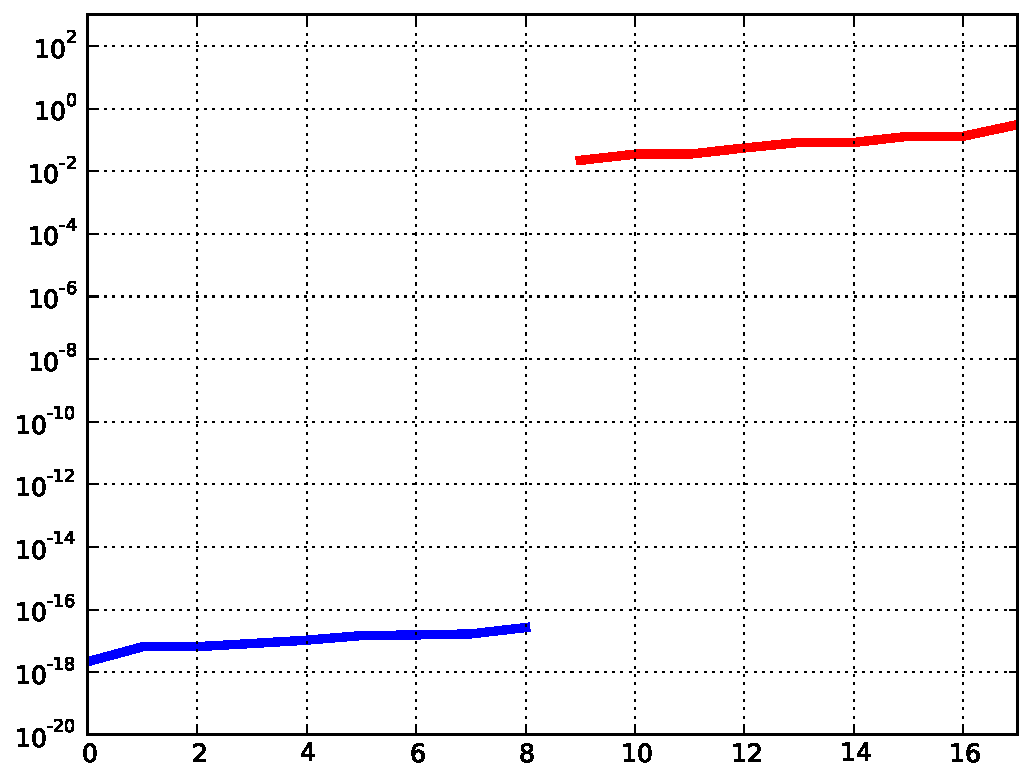
\includegraphics[width=5cm]{figs/shearlets/eigs/shl_dbl_nper_mass0}
& 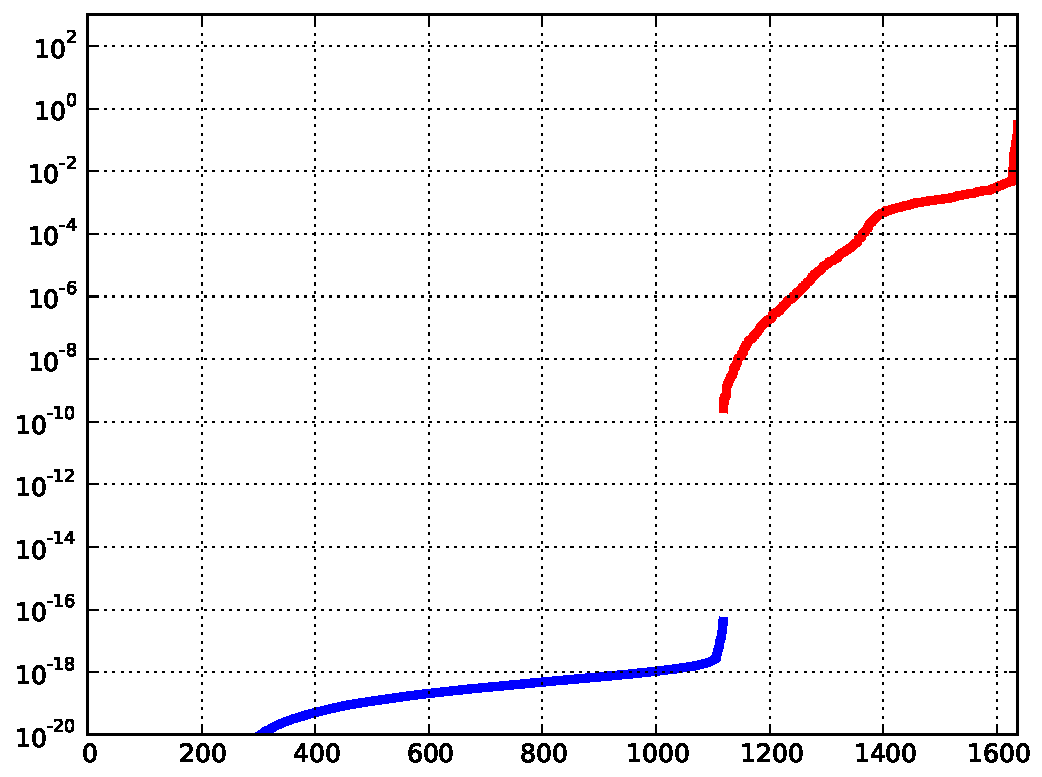
\includegraphics[width=5cm]{figs/shearlets/eigs/shl_dbl_nper_mass1} \\
\rotatebox{90}{\hspace{1.1cm}Transport}
  & 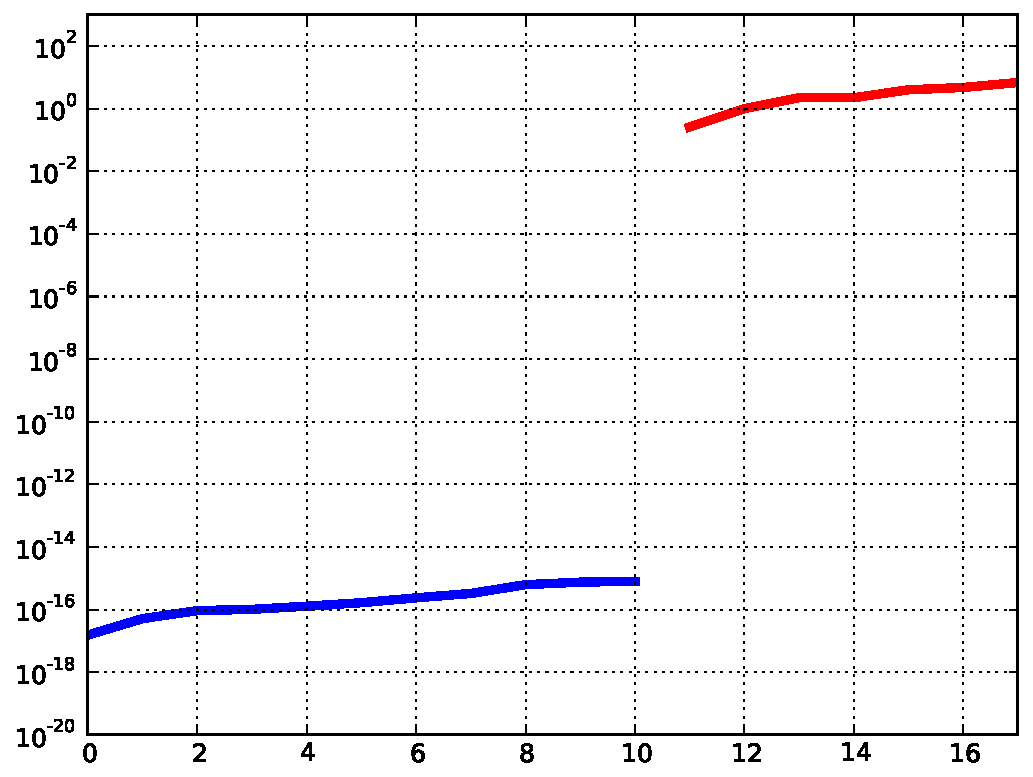
\includegraphics[width=5cm]{figs/shearlets/eigs/shl_dbl_nper_tran0}
  & 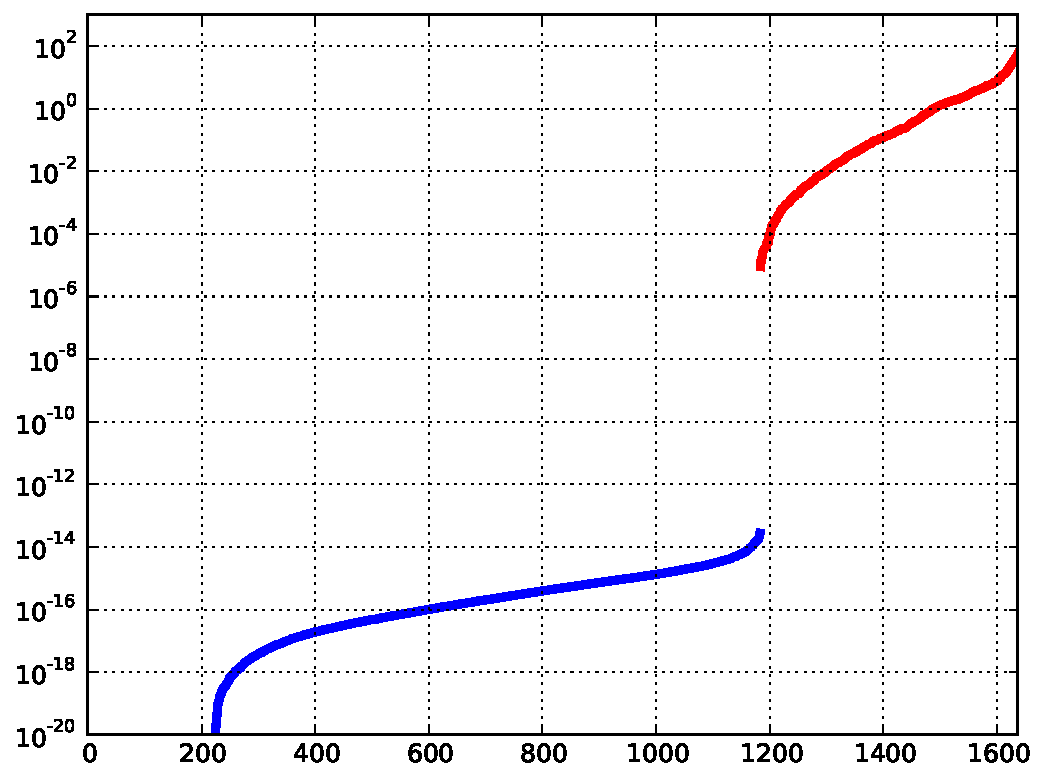
\includegraphics[width=5cm]{figs/shearlets/eigs/shl_dbl_nper_tran1}
\end{tabular}
\caption{Non-periodic, $(s_x,s_y)=(4,2)$.}
\label{fig:shl_dbl_nper}
\end{figure}

\begin{figure}
\centering
\begin{tabular}{ccc}
& $j=0$ & $j=1$ \\
\rotatebox{90}{\hspace{1.4cm}Mass} 
& 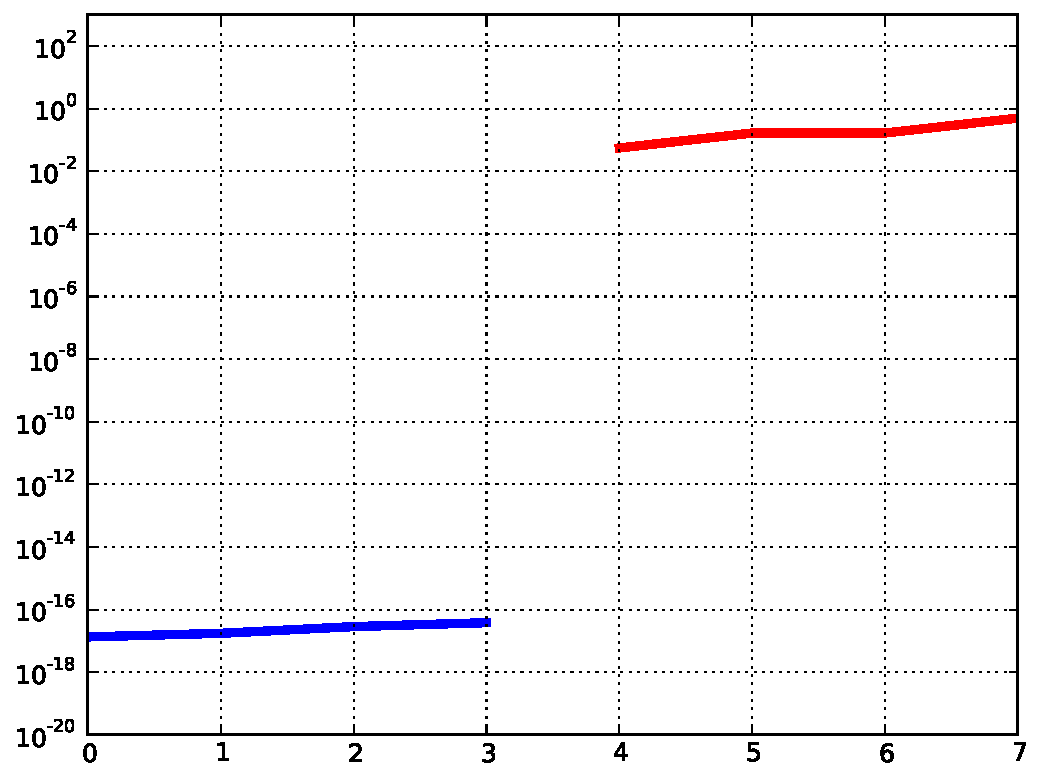
\includegraphics[width=5cm]{figs/shearlets/eigs/shl_dbl_per_mass0}
& 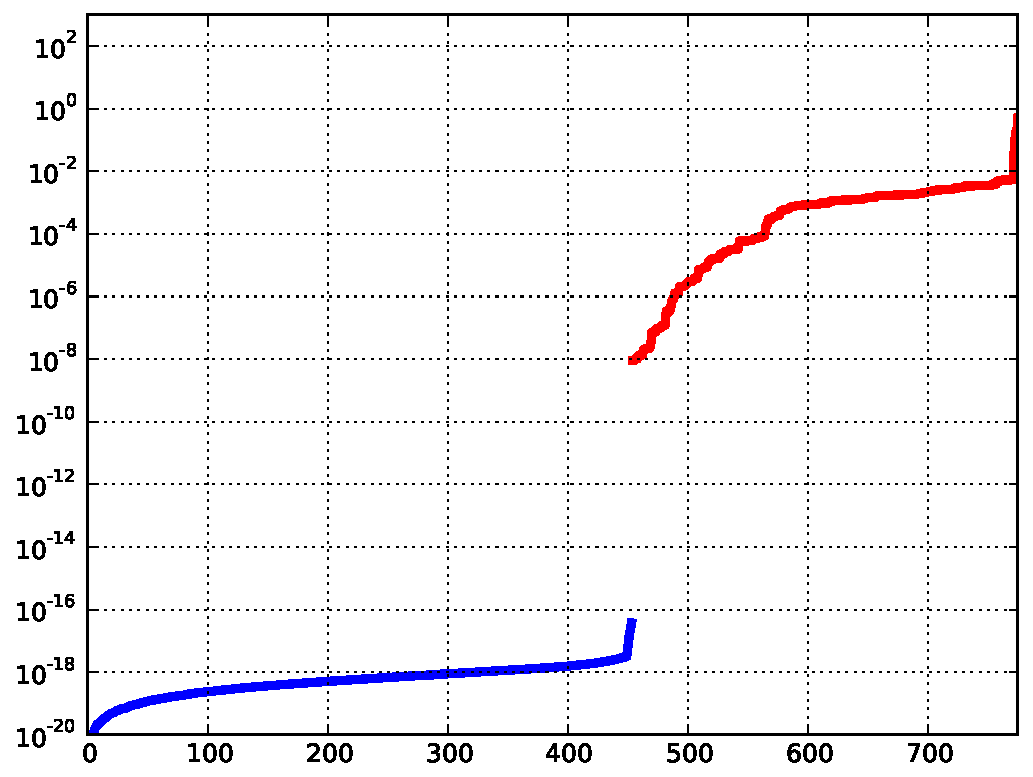
\includegraphics[width=5cm]{figs/shearlets/eigs/shl_dbl_per_mass1} \\
\rotatebox{90}{\hspace{1.1cm}Transport}
& 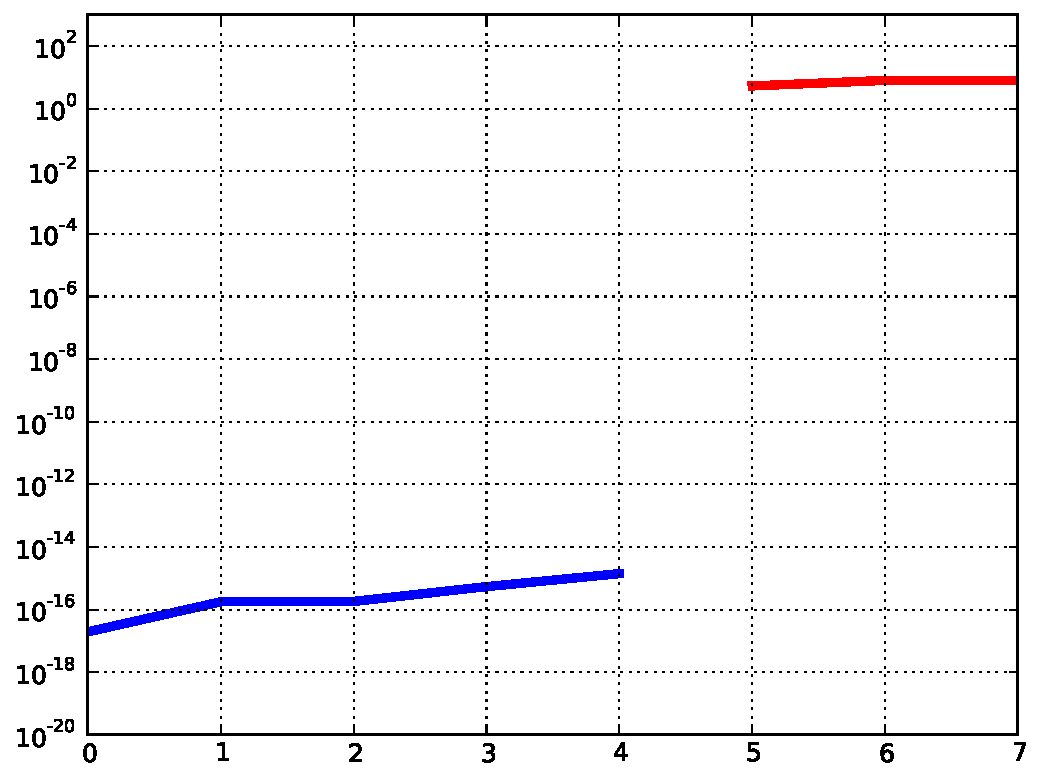
\includegraphics[width=5cm]{figs/shearlets/eigs/shl_dbl_per_tran0}
& 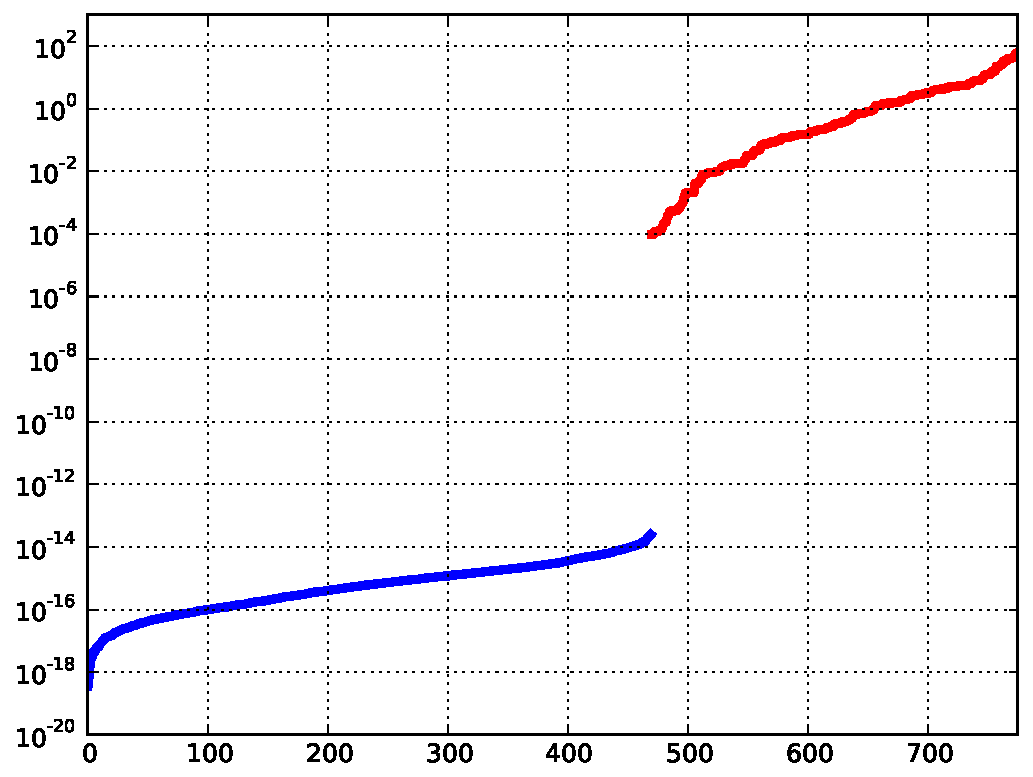
\includegraphics[width=5cm]{figs/shearlets/eigs/shl_dbl_per_tran1}
\end{tabular}
\caption{Periodic, $(s_x,s_y)=(4,2)$.}
\label{fig:shl_dbl_per}
\end{figure}

\begin{figure}
\hspace{-1.3cm}
\centering
\begin{tabular}{cccc}
& $j=0$ & $j=1$ & $j=2$ \\
\rotatebox{90}{\hspace{1.1cm}Mass} 
& 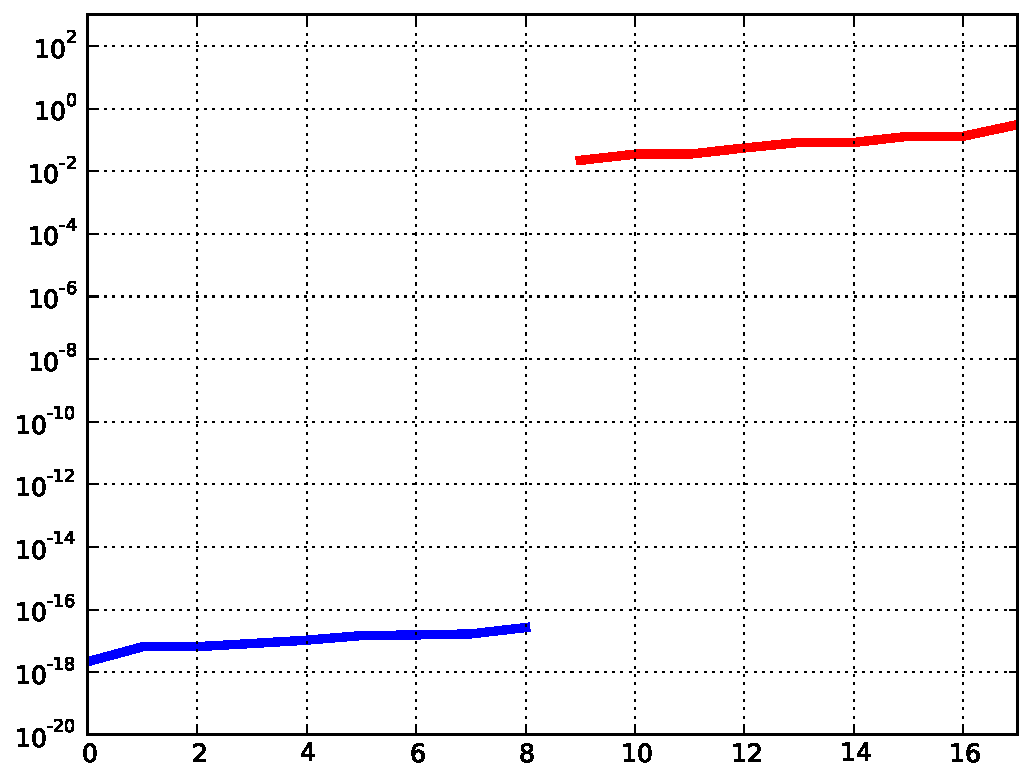
\includegraphics[width=4cm]{figs/shearlets/eigs/rid_dbl_nper_mass0}
& 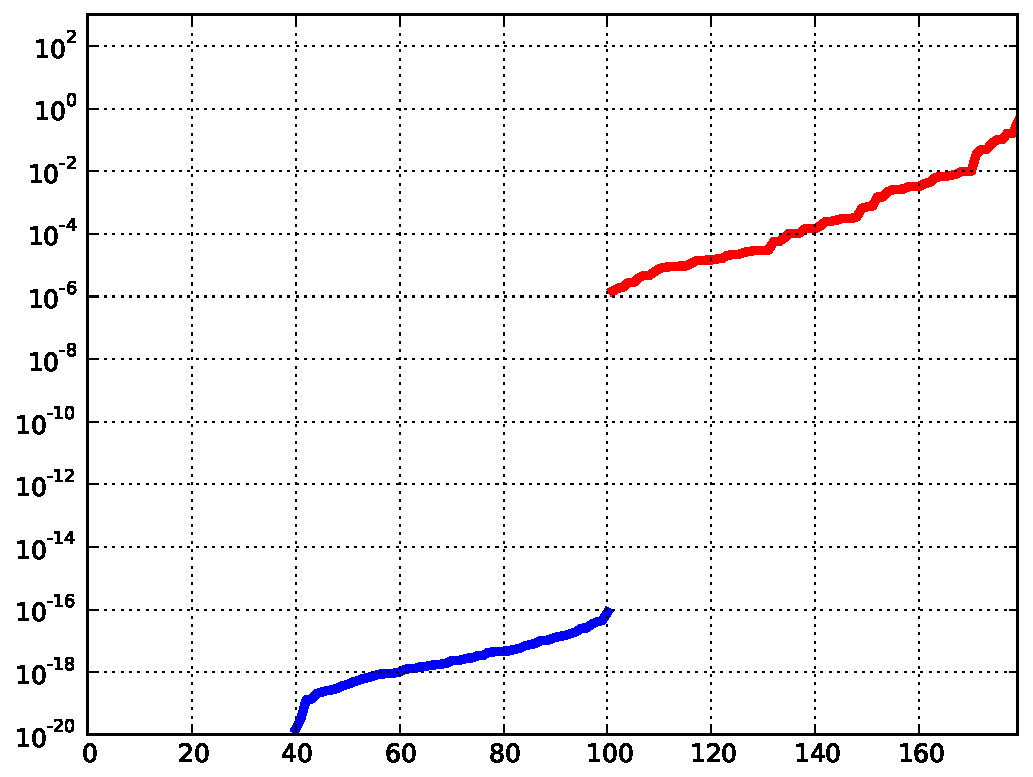
\includegraphics[width=4cm]{figs/shearlets/eigs/rid_dbl_nper_mass1}
& 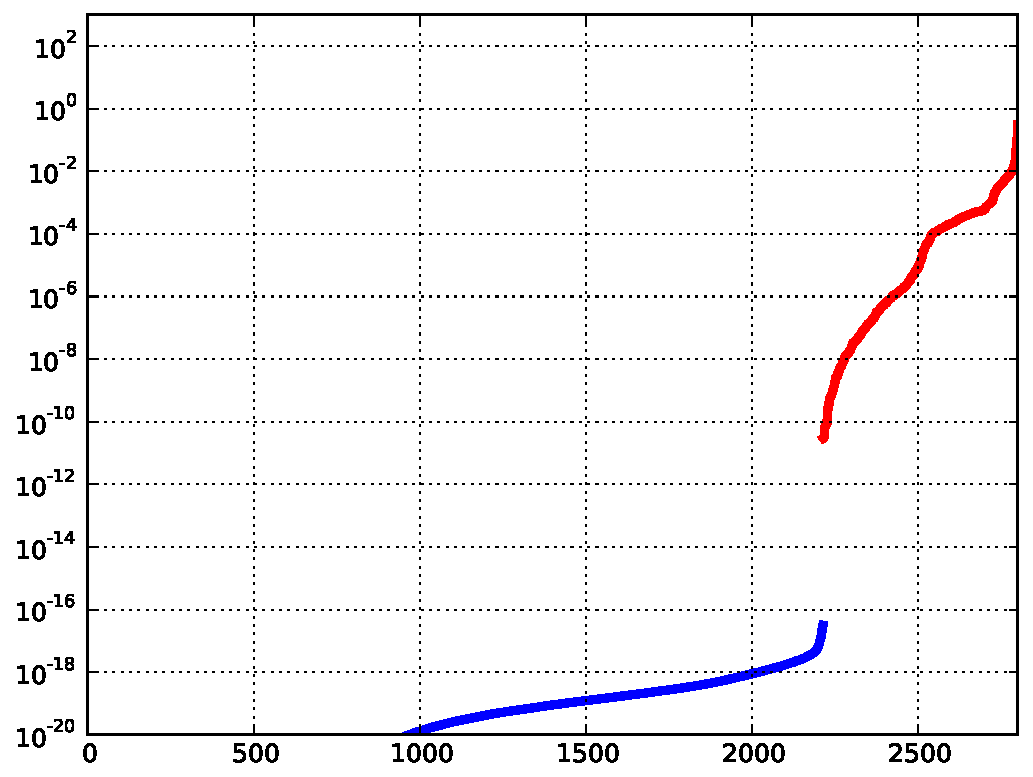
\includegraphics[width=4cm]{figs/shearlets/eigs/rid_dbl_nper_mass2} \\
\rotatebox{90}{\hspace{0.7cm}Transport}
& 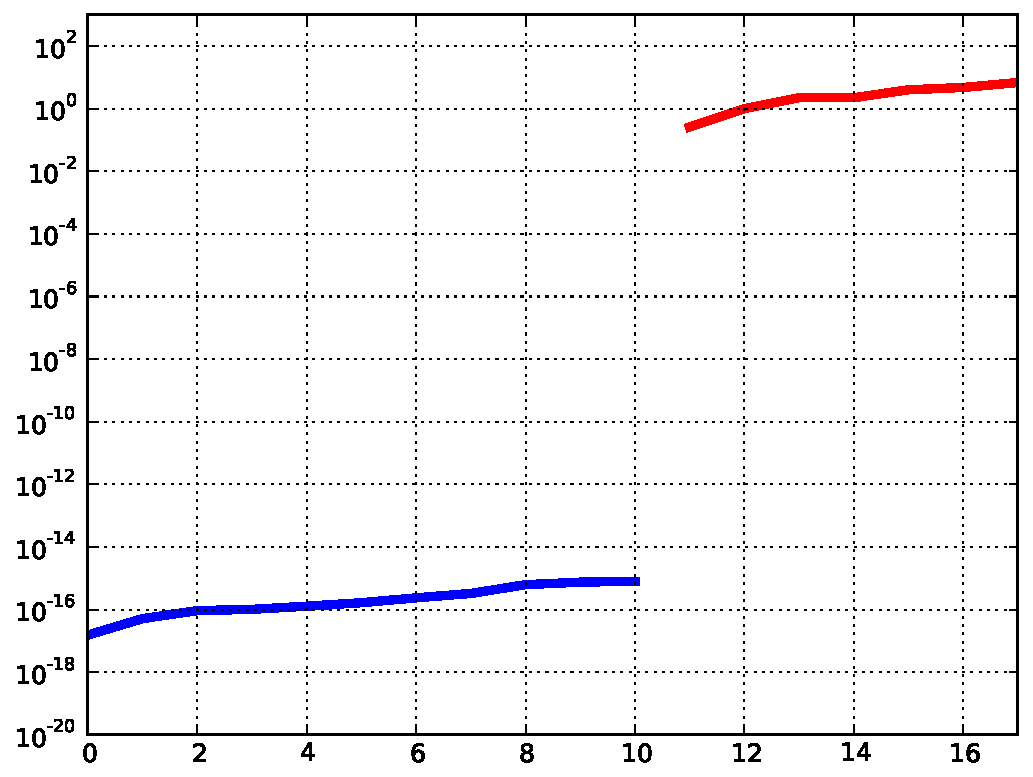
\includegraphics[width=4cm]{figs/shearlets/eigs/rid_dbl_nper_tran0}
& 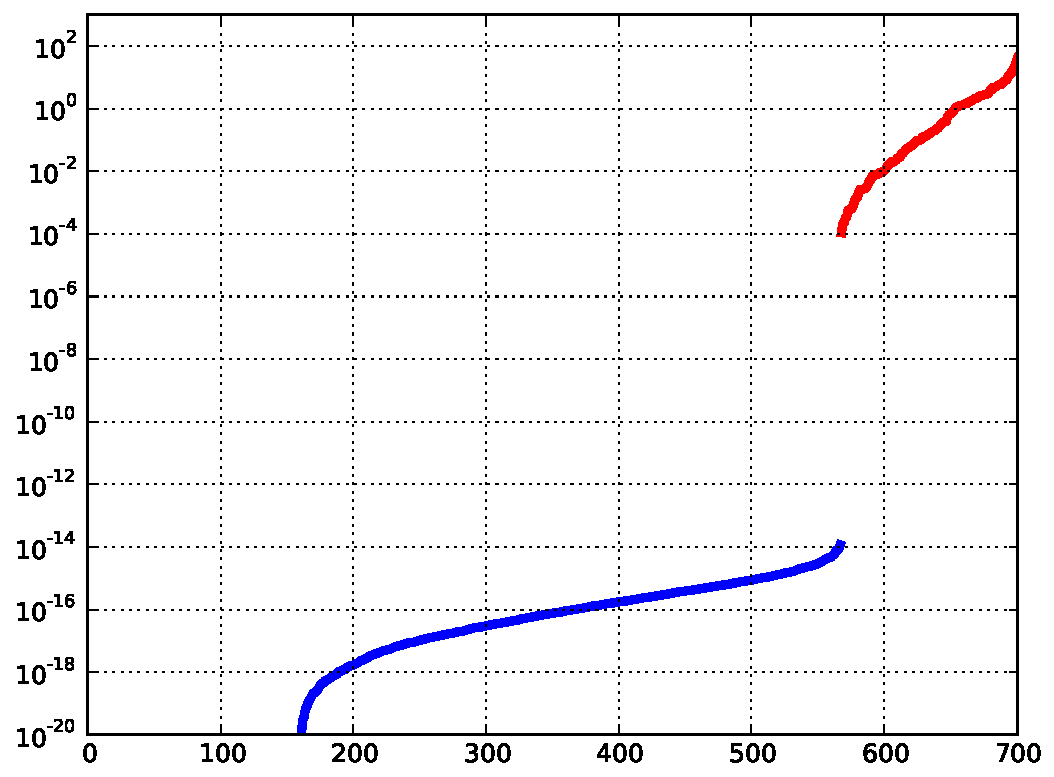
\includegraphics[width=4cm]{figs/shearlets/eigs/rid_dbl_nper_tran1}
& 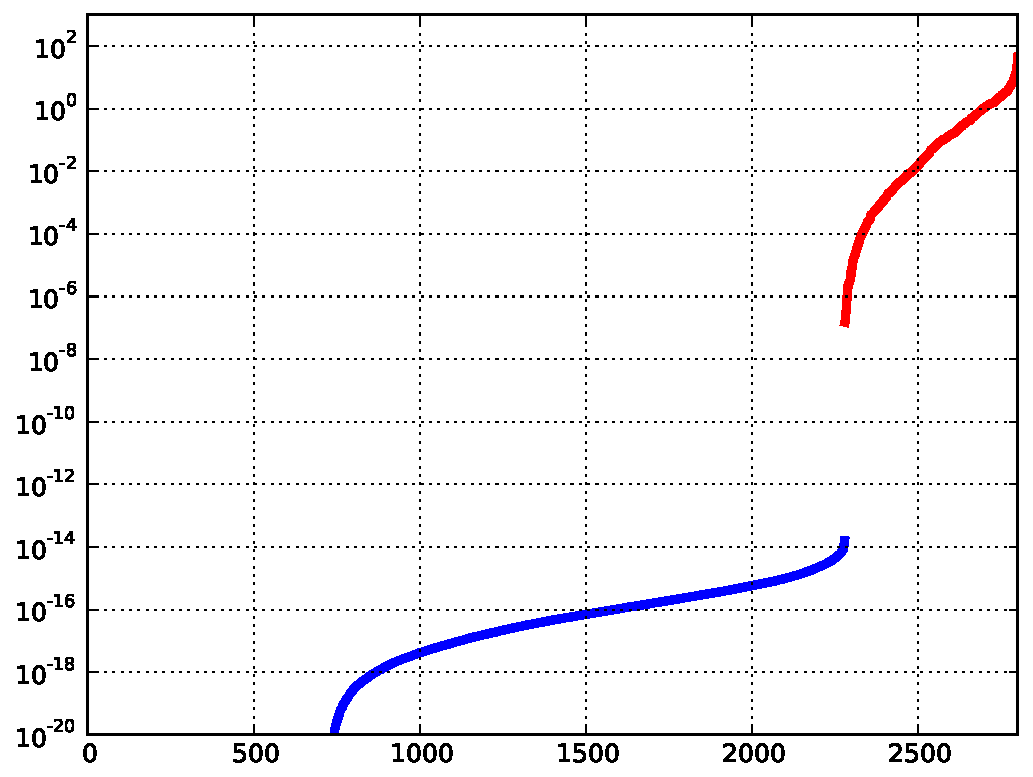
\includegraphics[width=4cm]{figs/shearlets/eigs/rid_dbl_nper_tran2}
\end{tabular}
\caption{Non-periodic, $(s_x,s_y)=(2,1)$.}
\label{fig:rid_dbl_nper}
\end{figure}

\begin{figure}
\hspace{-1.3cm}
\centering
\begin{tabular}{cccc}
& $j=0$ & $j=1$ & $j=2$ \\
\rotatebox{90}{\hspace{1.1cm}Mass} 
& 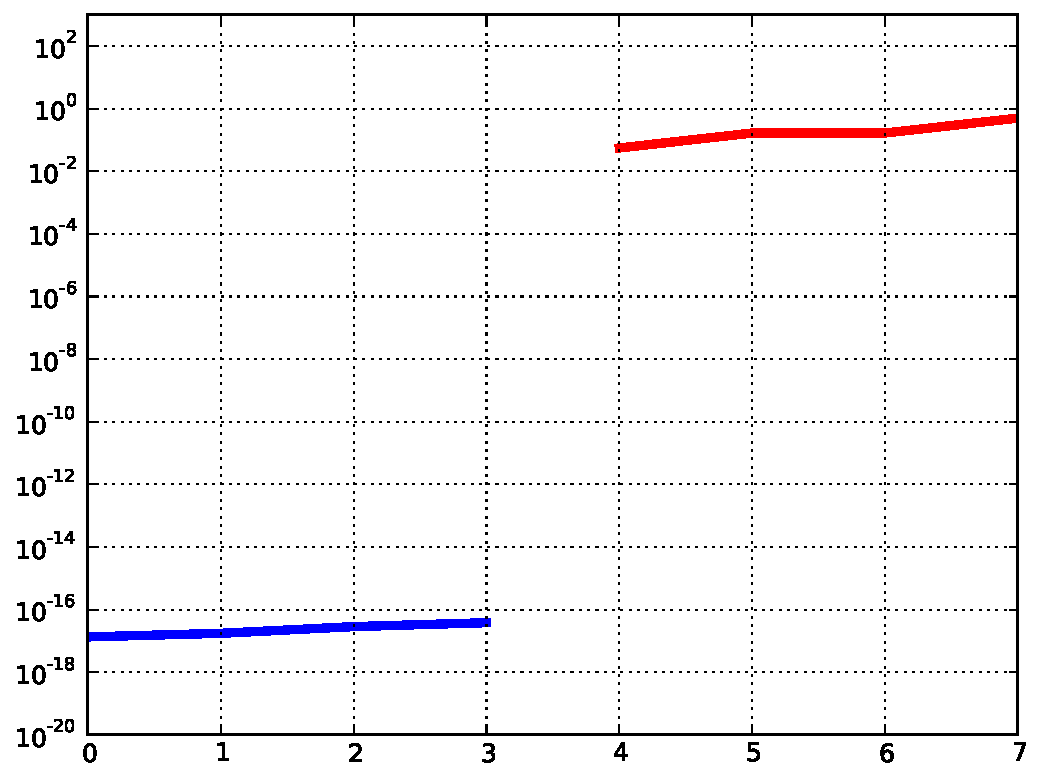
\includegraphics[width=4cm]{figs/shearlets/eigs/rid_dbl_per_mass0}
& 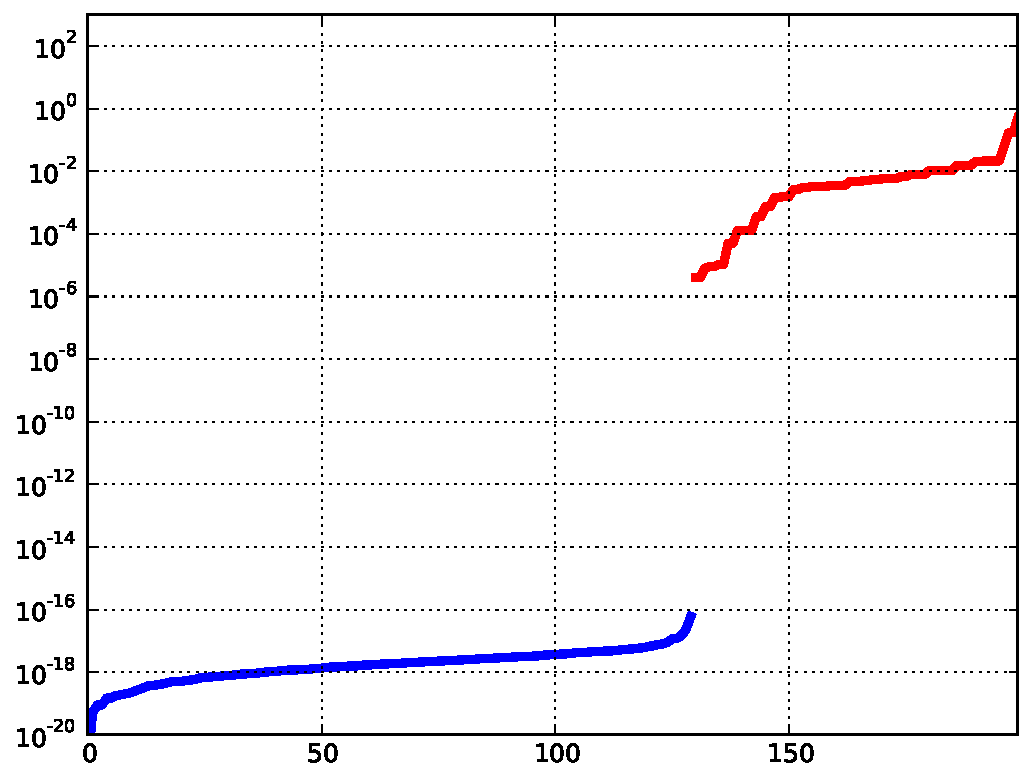
\includegraphics[width=4cm]{figs/shearlets/eigs/rid_dbl_per_mass1}
& 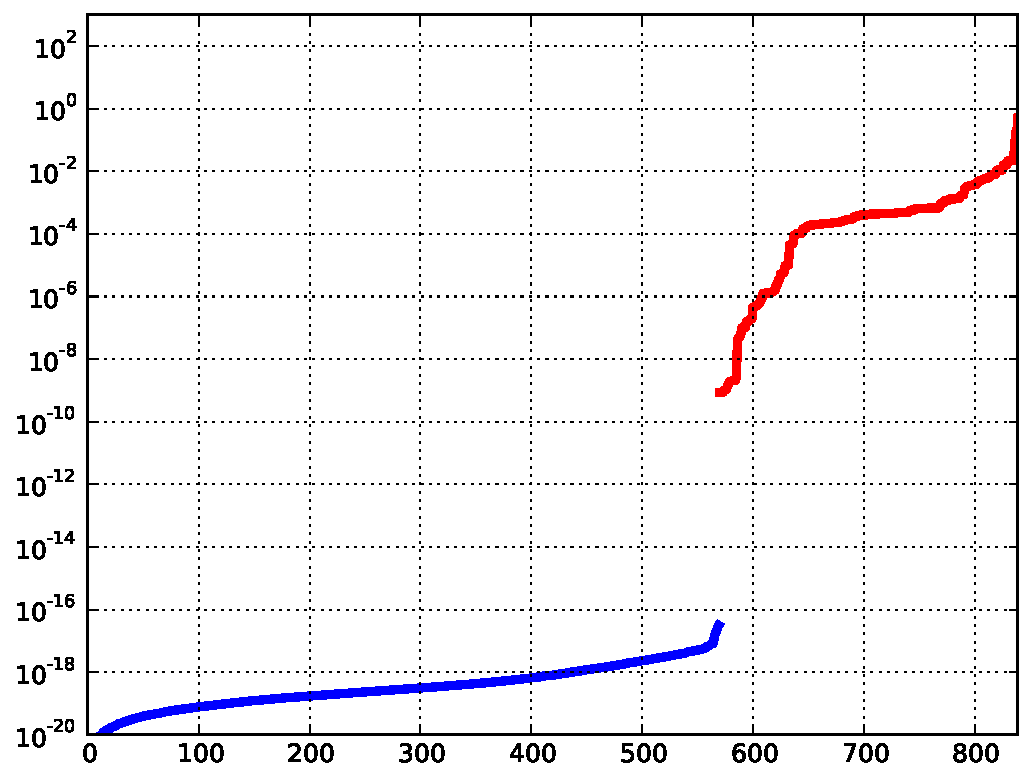
\includegraphics[width=4cm]{figs/shearlets/eigs/rid_dbl_per_mass2} \\
\rotatebox{90}{\hspace{0.7cm}Transport}
& 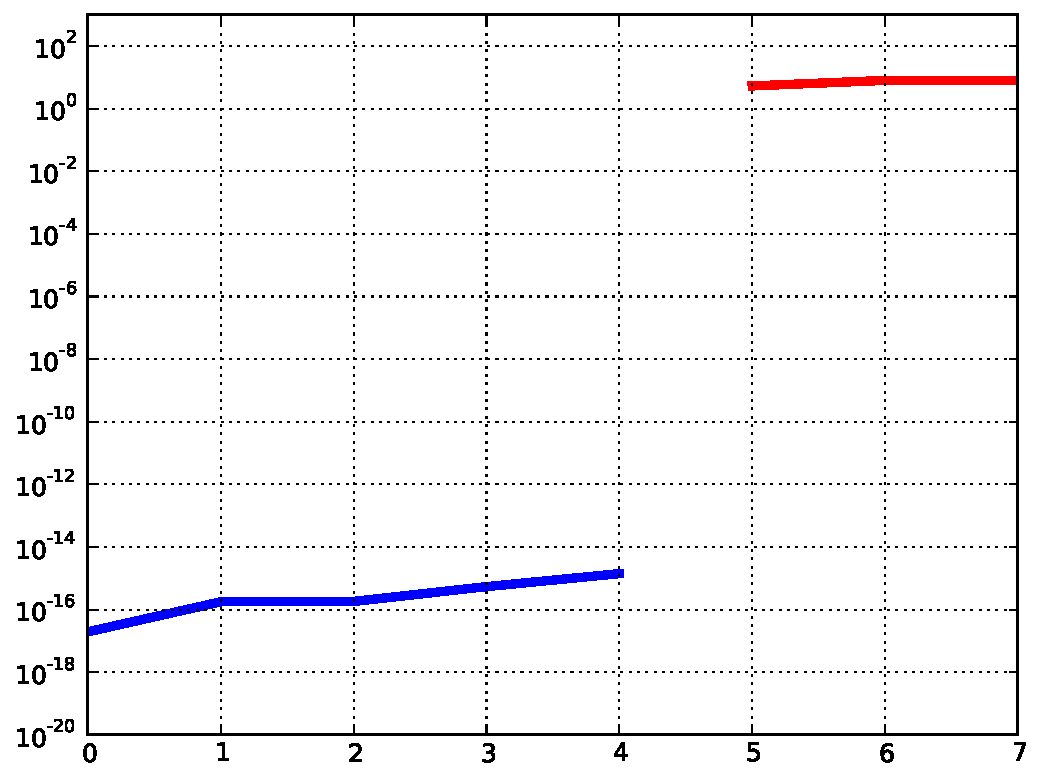
\includegraphics[width=4cm]{figs/shearlets/eigs/rid_dbl_per_tran0}
& 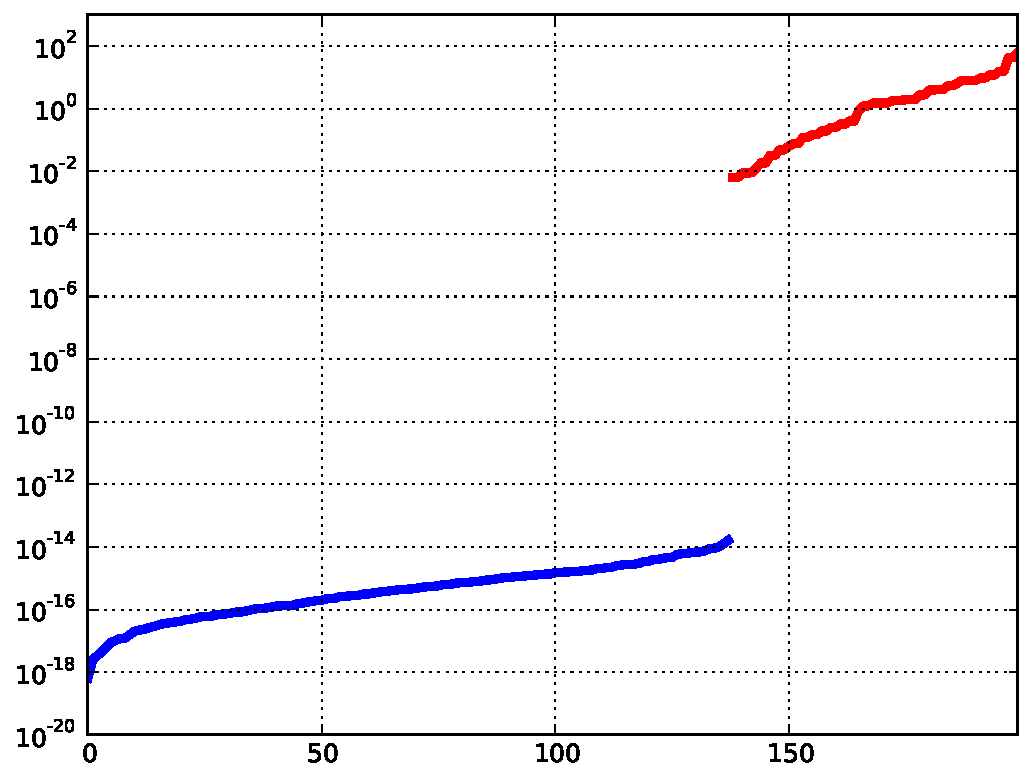
\includegraphics[width=4cm]{figs/shearlets/eigs/rid_dbl_per_tran1}
& 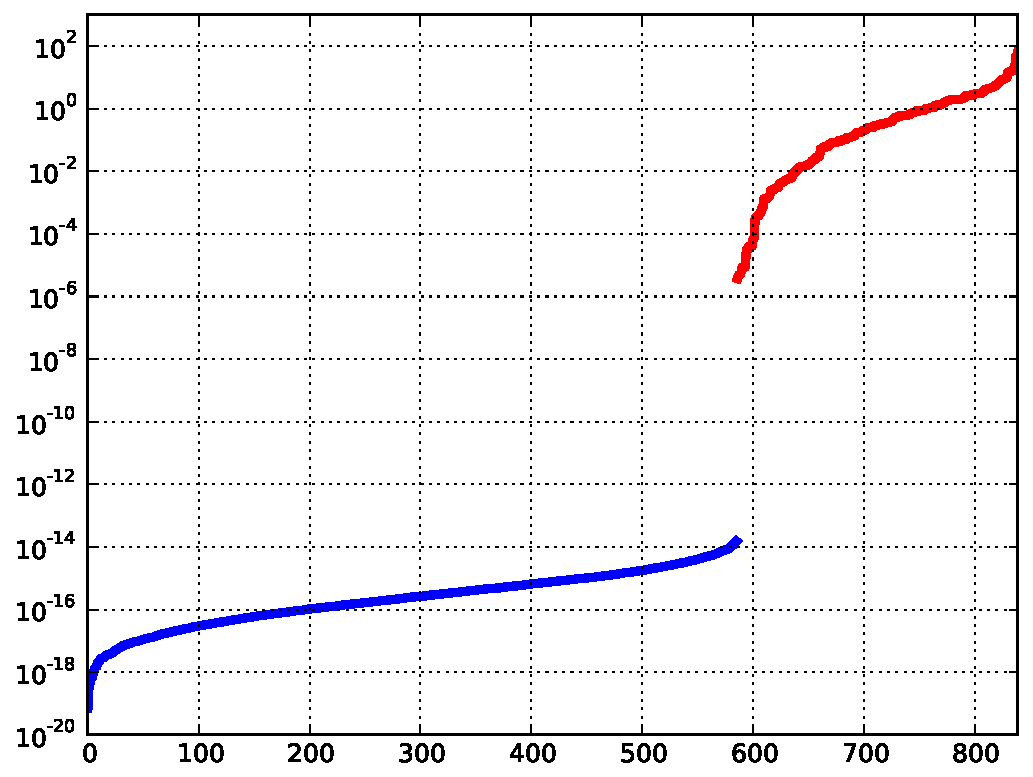
\includegraphics[width=4cm]{figs/shearlets/eigs/rid_dbl_per_tran2}
\end{tabular}
\caption{Periodic, $(s_x,s_y)=(2,1)$.}
\label{fig:rid_dbl_per}
\end{figure}

\begin{figure}
\hspace{-1.3cm}
\centering
\begin{tabular}{cccc}
& $j=0$ & $j=1$ & $j=2$ \\
\rotatebox{90}{\hspace{1.1cm}Mass} 
& 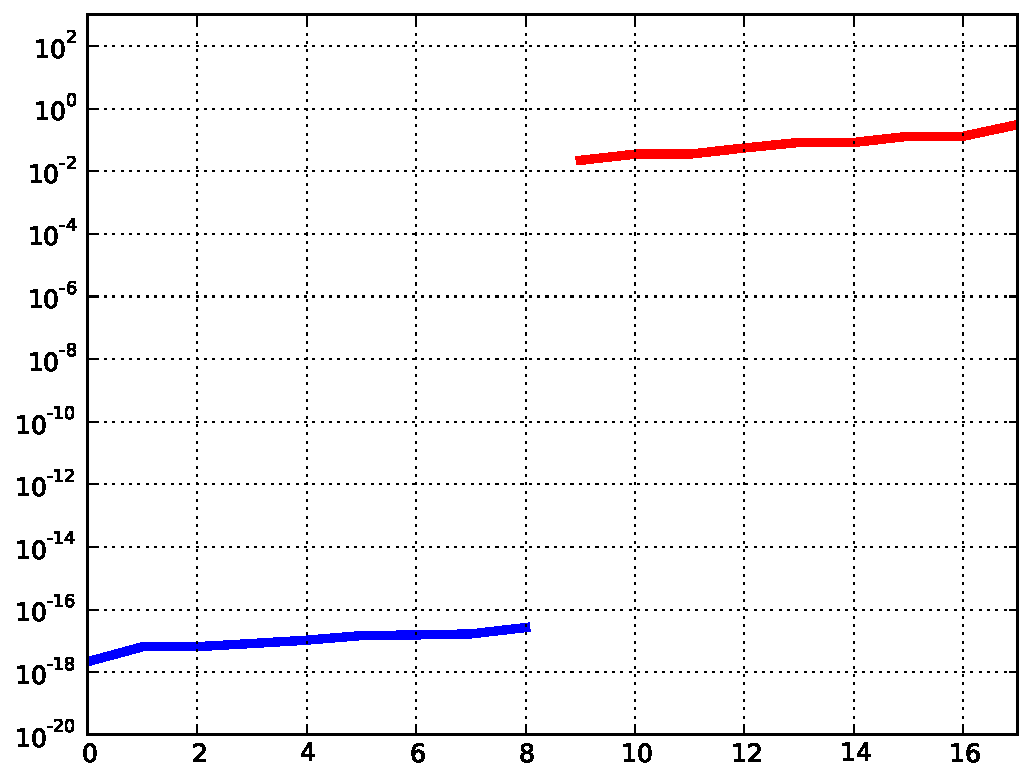
\includegraphics[width=4cm]{figs/shearlets/eigs/rid_sglhat_nper_mass0}
& 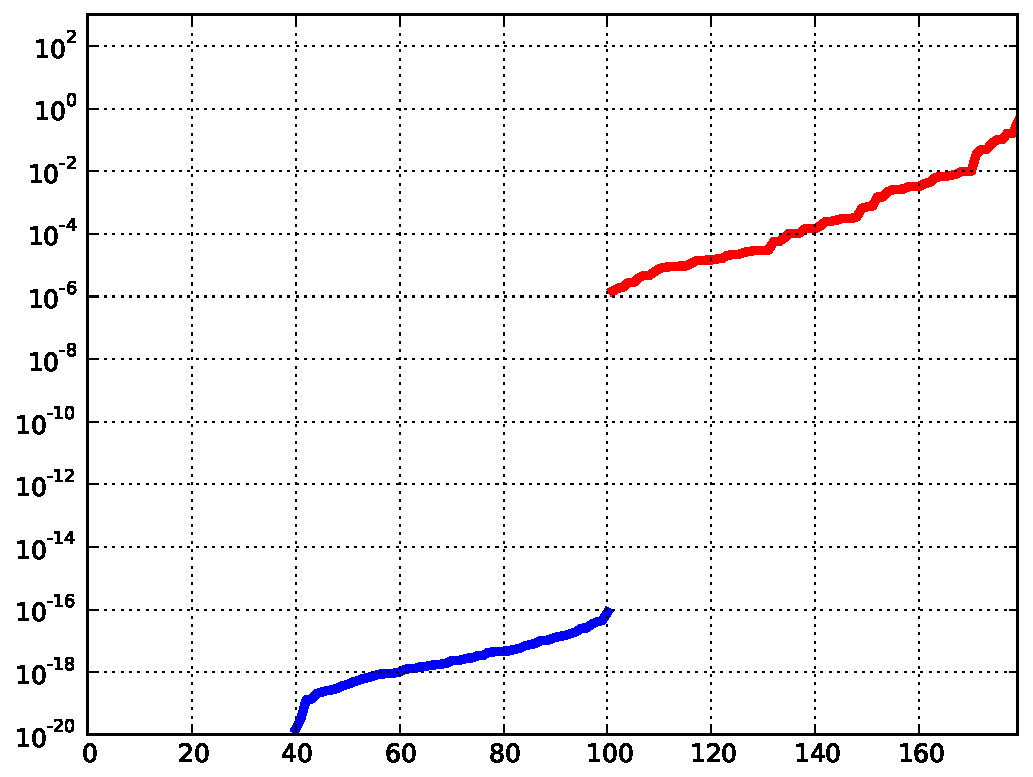
\includegraphics[width=4cm]{figs/shearlets/eigs/rid_sglhat_nper_mass1}
& 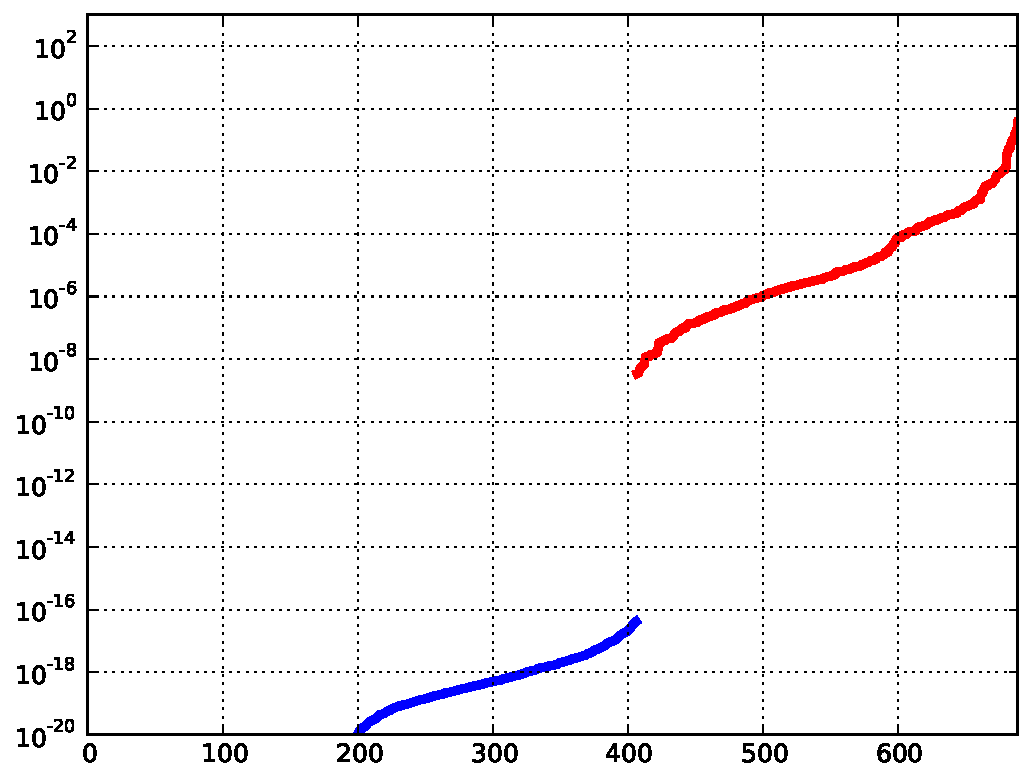
\includegraphics[width=4cm]{figs/shearlets/eigs/rid_sglhat_nper_mass2} \\
\rotatebox{90}{\hspace{0.7cm}Transport}
& 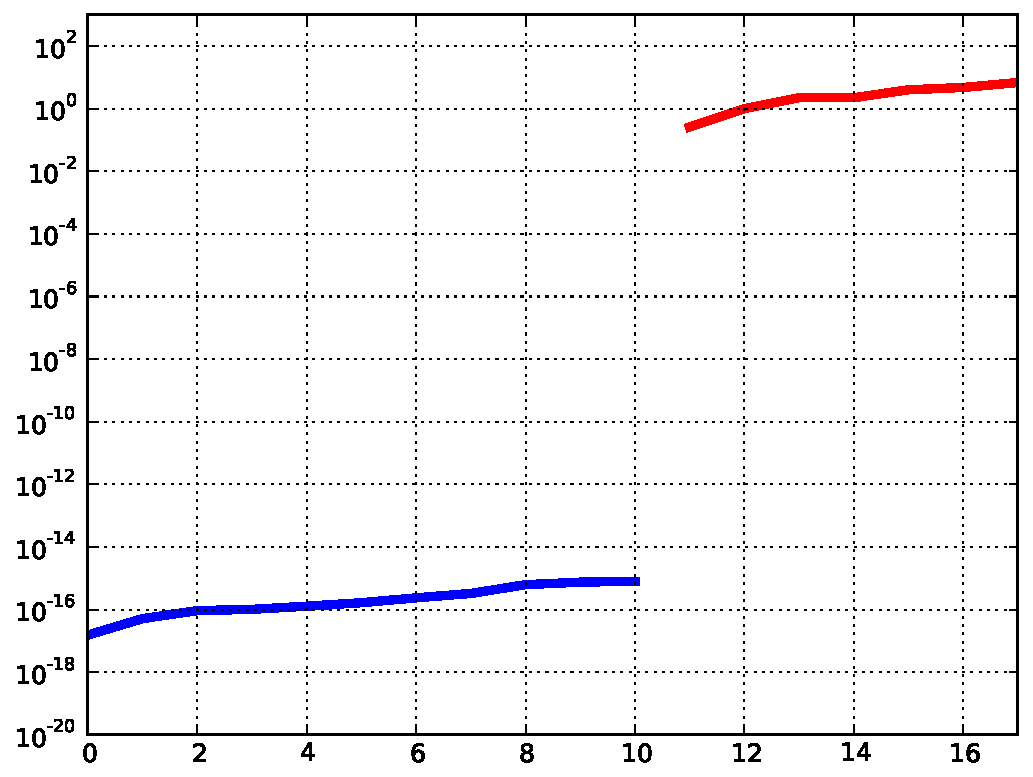
\includegraphics[width=4cm]{figs/shearlets/eigs/rid_sglhat_nper_tran0}
& 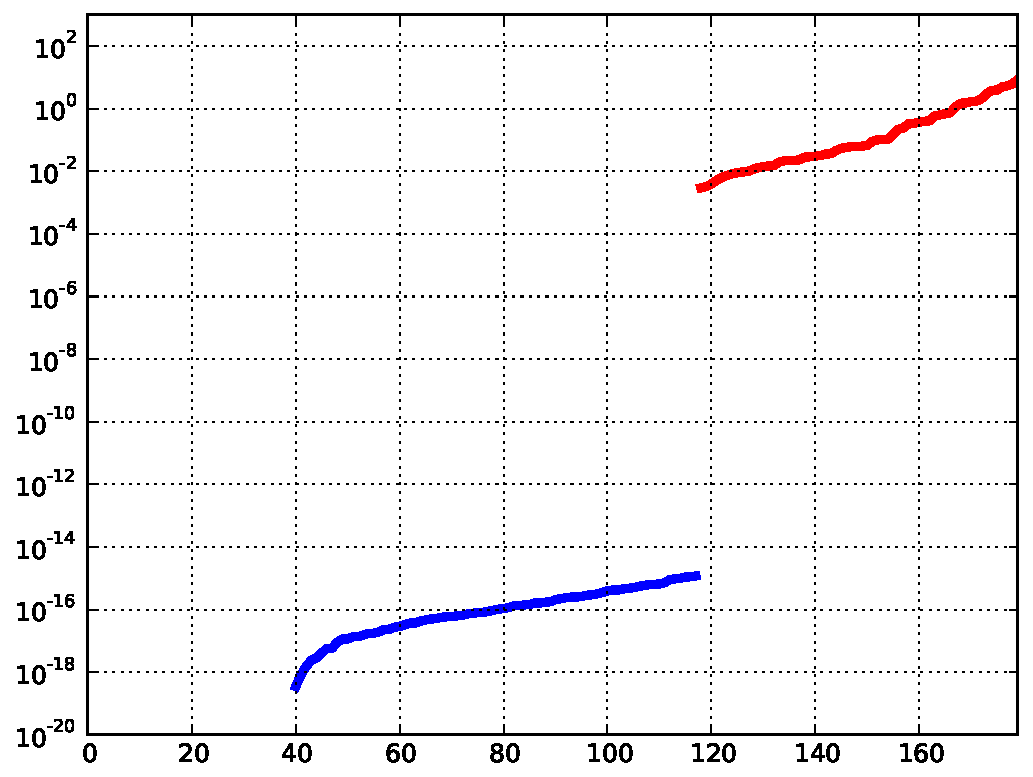
\includegraphics[width=4cm]{figs/shearlets/eigs/rid_sglhat_nper_tran1}
& 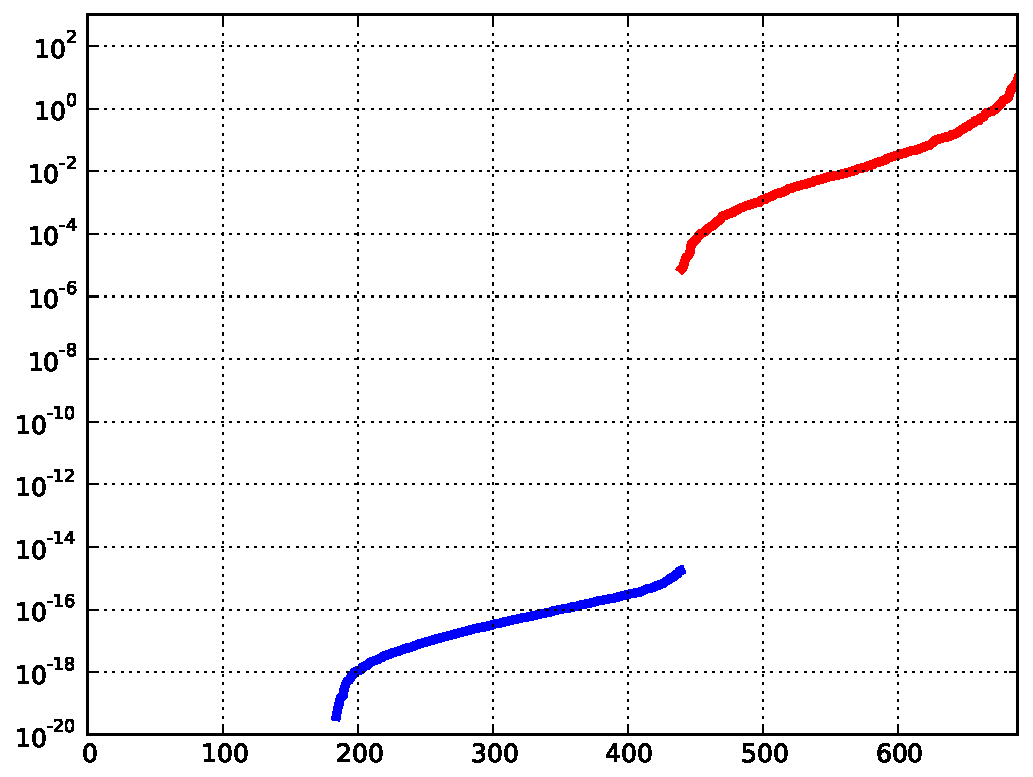
\includegraphics[width=4cm]{figs/shearlets/eigs/rid_sglhat_nper_tran2}
\end{tabular}
\caption{Non-periodic hat functions, $(s_x,s_y)=(2,1)$.}
\label{fig:rid_sglhat_nper}
\end{figure}

\begin{figure}
\hspace{-1.3cm}
\centering
\begin{tabular}{cccc}
& $j=0$ & $j=1$ & $j=2$ \\
\rotatebox{90}{\hspace{1.1cm}Mass} 
& 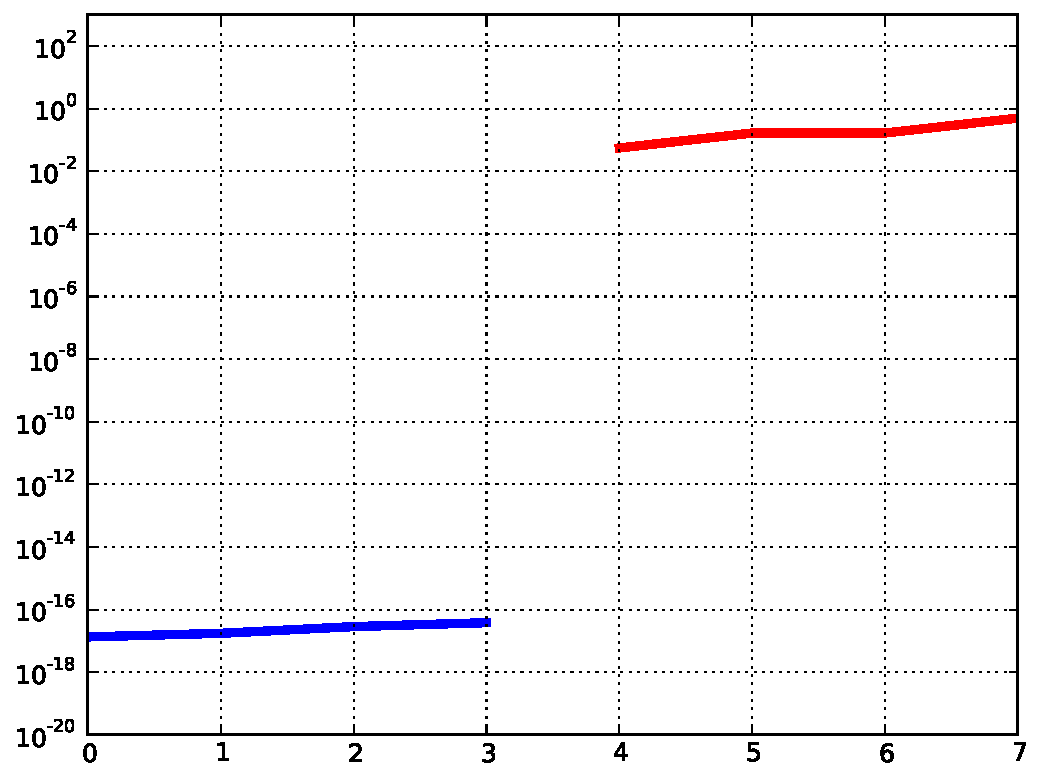
\includegraphics[width=4cm]{figs/shearlets/eigs/rid_sglhat_per_mass0}
& 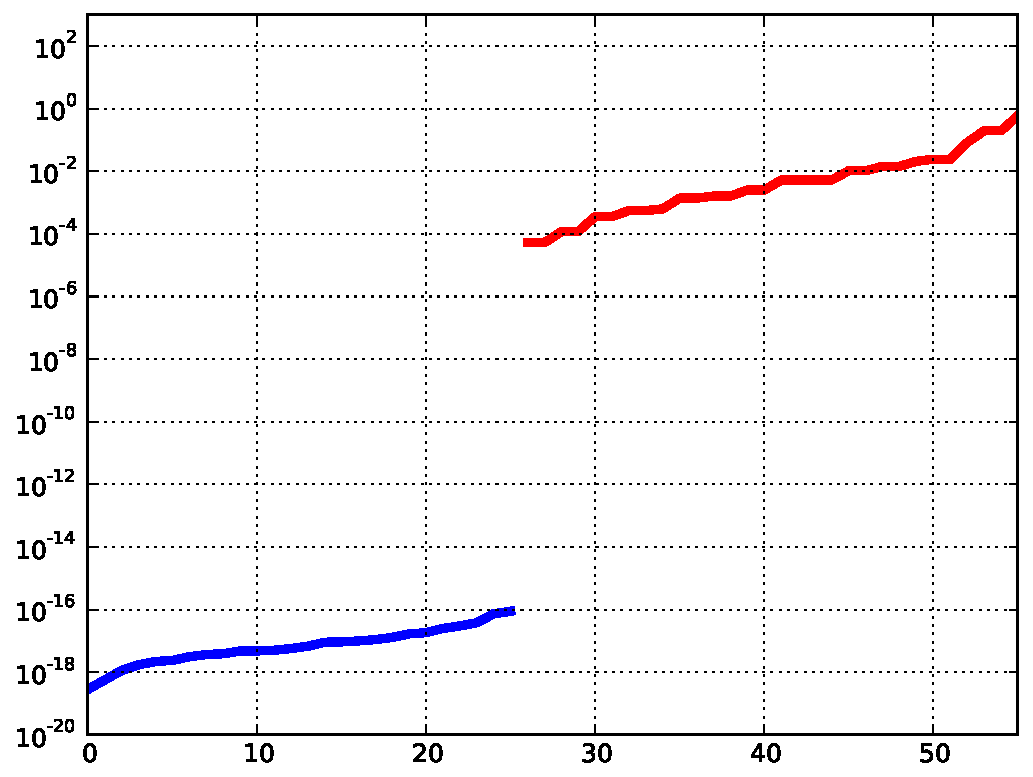
\includegraphics[width=4cm]{figs/shearlets/eigs/rid_sglhat_per_mass1}
& 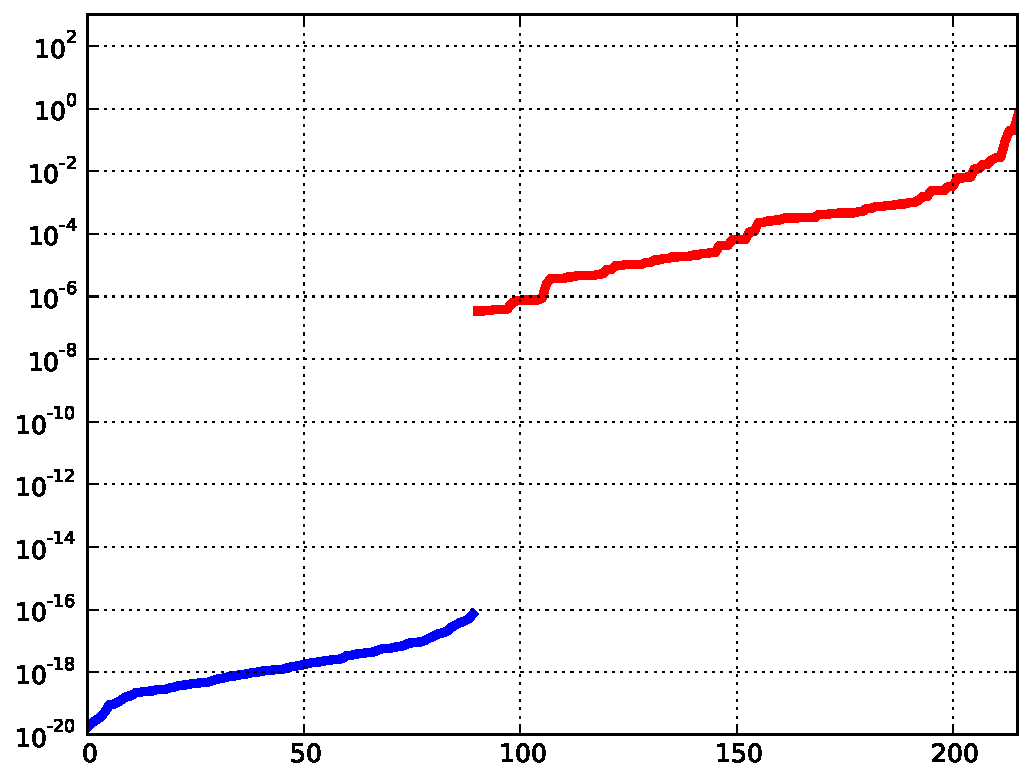
\includegraphics[width=4cm]{figs/shearlets/eigs/rid_sglhat_per_mass2} \\
\rotatebox{90}{\hspace{0.7cm}Transport}
& 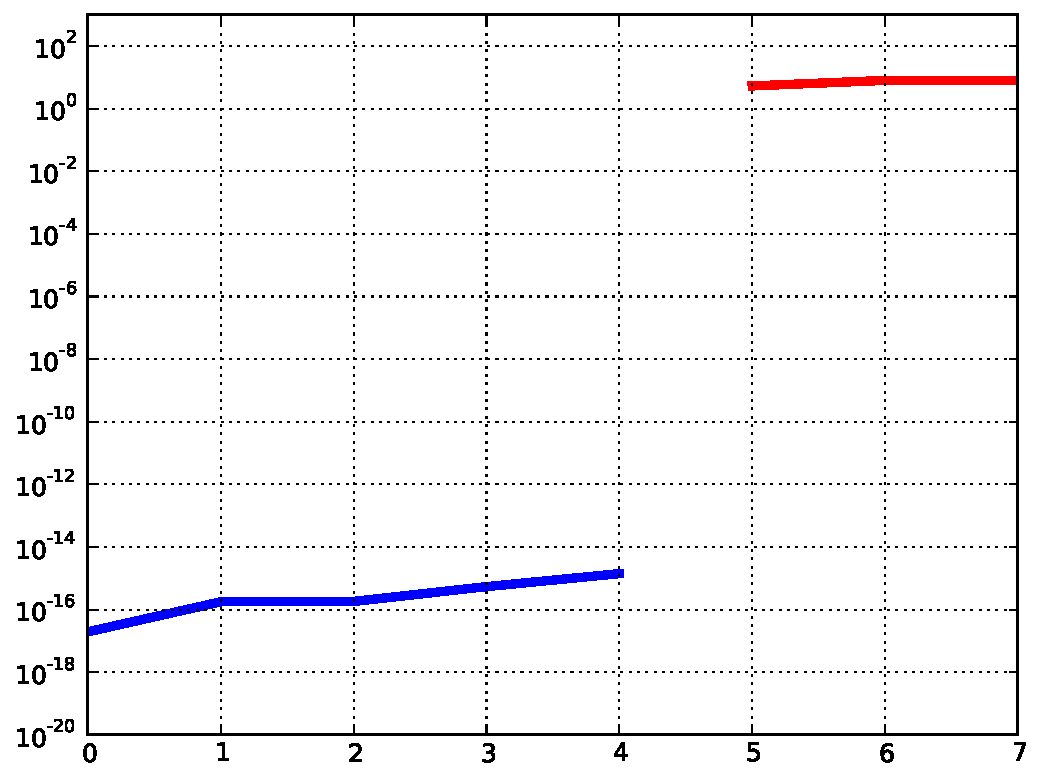
\includegraphics[width=4cm]{figs/shearlets/eigs/rid_sglhat_per_tran0}
& 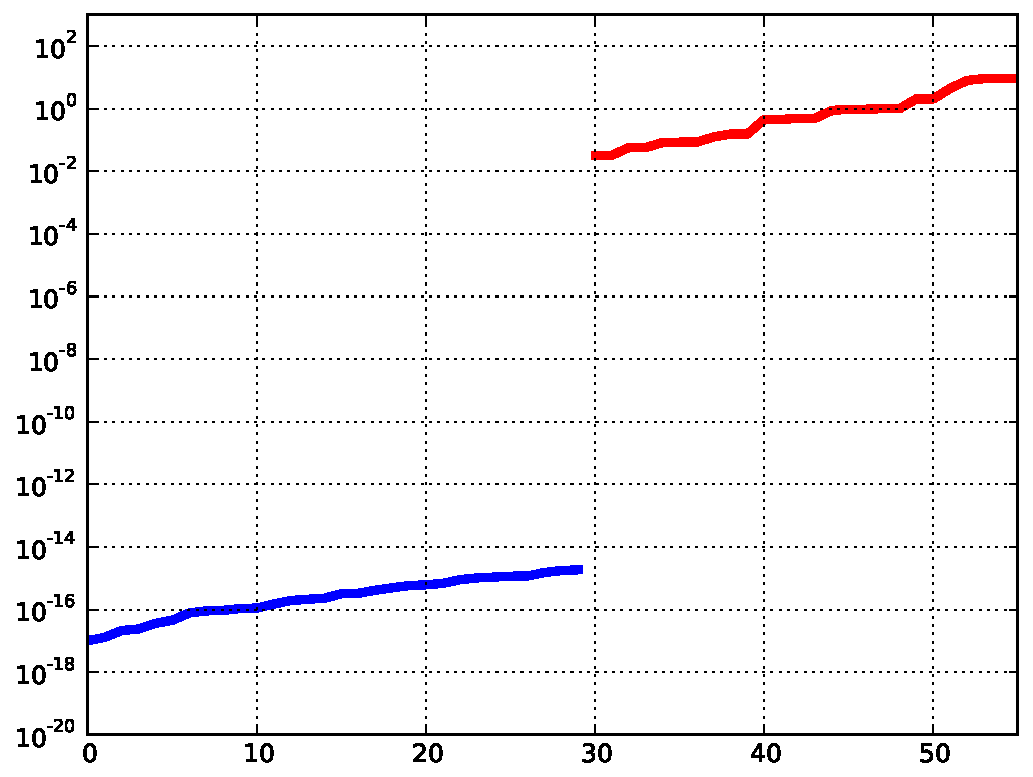
\includegraphics[width=4cm]{figs/shearlets/eigs/rid_sglhat_per_tran1}
& 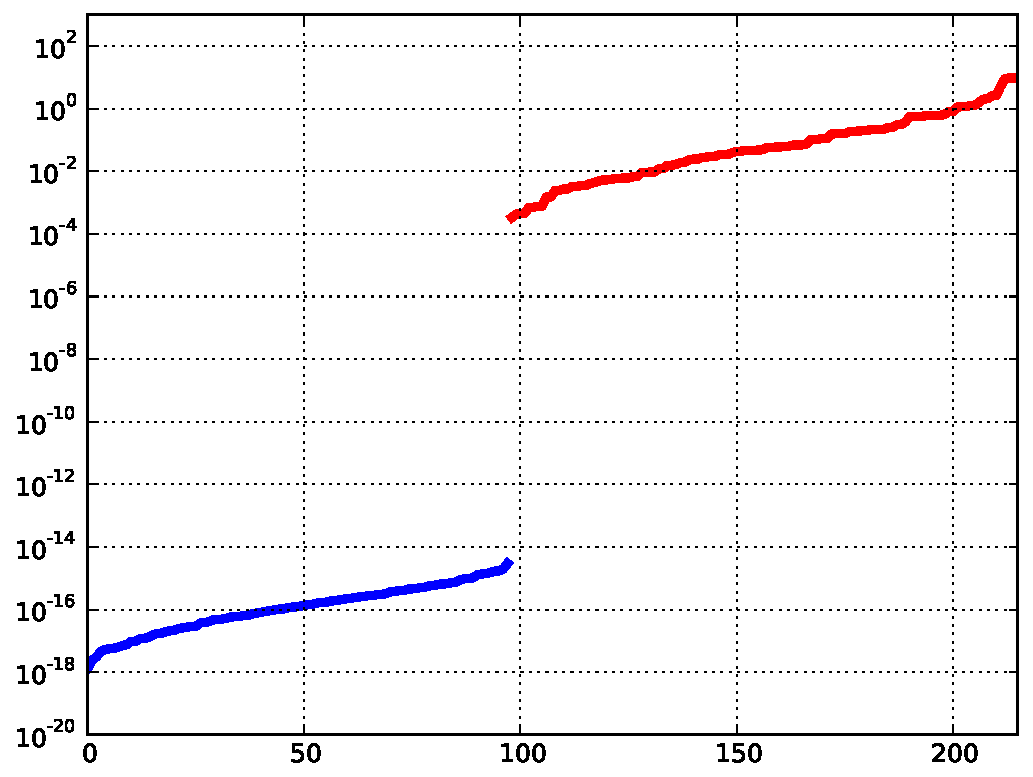
\includegraphics[width=4cm]{figs/shearlets/eigs/rid_sglhat_per_tran2}
\end{tabular}
\caption{Periodic hat functions, $(s_x,s_y)=(2,1)$.}
\label{fig:rid_sglhat_per}
\end{figure}

\begin{landscape}
\begin{table}
\centering
\def\arraystretch{1.2}
\begin{tabular}{ccccccccc}
$s_x$ & $s_y$ & Periodic & Mothers & Matrix & $j=0$ & $j=1$ & $j=2$ & $j=3$ \\
\hline \noalign{\vskip 1mm} 
$4$ & $2$ & No & Normal & Mass & $1.39\cdot10^1$ & $1.19\cdot10^9$ & & \\
\hline \noalign{\vskip 1mm}
$4$ & $2$ & No & Normal & Transport & $2.61\cdot10^1$ & $6.24\cdot10^6$ & & \\
\hline \noalign{\vskip 1mm}
$4$ & $2$ & Yes & Normal & Mass & $9.00\cdot10^0$ & $5.66\cdot10^7$ & & \\
\hline \noalign{\vskip 1mm}
$4$ & $2$ & Yes & Normal & Transport & $1.50\cdot10^0$ & $6.83\cdot10^5$ & & \\
\hline \noalign{\vskip 1mm} 
$2$ & $1$ & No & Normal & Mass & $1.39\cdot10^1$ & $2.51\cdot10^5$ & $1.05\cdot10^{10}$ & \\
\hline \noalign{\vskip 1mm}
$2$ & $1$ & No & Normal & Transport & $2.61\cdot10^1$ & $3.99\cdot10^5$ & $3.02\cdot10^8$ & \\
\hline \noalign{\vskip 1mm}
$2$ & $1$ & Yes & Normal & Mass & $9.00\cdot10^0$ & $1.23\cdot10^5$ & $5.73\cdot10^8$ & \\
\hline \noalign{\vskip 1mm}
$2$ & $1$ & Yes & Normal & Transport & $1.50\cdot10^0$ & $1.02\cdot10^4$ & $1.79\cdot10^7$ & \\
\hline \noalign{\vskip 1mm} 
$2$ & $1$ & No & Single & Mass & $1.39\cdot10^1$ & $2.51\cdot10^5$ & $1.10\cdot10^8$ & $2.61\cdot10^{11}$ \\
\hline \noalign{\vskip 1mm}
$2$ & $1$ & No & Single & Transport & $2.61\cdot10^1$ & $2.92\cdot10^3$ & $1.15\cdot10^6$ & $6.76\cdot10^8$ \\
\hline \noalign{\vskip 1mm}
$2$ & $1$ & Yes & Single & Mass & $9.00\cdot10^0$ & $1.13\cdot10^4$ & $1.78\cdot10^6$ & $6.76\cdot10^8$ \\
\hline \noalign{\vskip 1mm}
$2$ & $1$ & Yes & Single & Transport & $1.50\cdot10^0$ & $2.87\cdot10^2$ & $2.88\cdot10^4$ & $7.41\cdot10^6$ \\
\end{tabular}
\caption{Effective condition numbers for all cases shown in Figure \ref{fig:shl_dbl_nper} through
\ref{fig:rid_sglhat_per}.}
\label{tbl:shletconds}
\end{table}
\end{landscape}
